\documentclass[10pt]{article}
\usepackage[utf8]{inputenc}
\usepackage[T1]{fontenc}
\usepackage{amsmath}
\usepackage{amsfonts}
\usepackage{amssymb}
\usepackage[version=4]{mhchem}
\usepackage{stmaryrd}
\usepackage{graphicx}
\usepackage[export]{adjustbox}
\graphicspath{ {./images/} }
\usepackage{times}  %Makes text TimesNewRoman
\usepackage{setspace} %Allows you to set single or double space 
\usepackage{biblatex} %Imports biblatex package
\usepackage{authblk}
\usepackage{subfig}
\usepackage{float}
\usepackage{tabularx}
\usepackage{multirow}
\usepackage[paperheight=11in,
   paperwidth=8.5in,
   top=20mm,
   bottom=20mm,
   left=40mm,
   right=40mm]{geometry}
\usepackage{moresize}
\usepackage{tikz}
\usepackage{xcolor}
\usepackage{physics}
\usepackage{amssymb}
\usepackage{mathrsfs}
\usepackage{amsmath}
\usepackage{ragged2e}
\usepackage{comment}
\usepackage{xcolor}
\usepackage[colorlinks=true, urlcolor=blue, linkcolor=blue]{hyperref}
\singlespacing  %Sets single spacing for whole document

%Bibliography Block
\addbibresource{QnotesCH1.bib}

%New command to display footnote whose markers will always be hidden
\let\svthefootnote\thefootnote
\newcommand\blfootnotetext[1]{%
  \let\thefootnote\relax\footnote{#1}%
  \addtocounter{footnote}{-1}%
  \let\thefootnote\svthefootnote%
}

%Overriding the \footnotetext command to hide the marker if its value is `0`
\let\svfootnotetext\footnotetext
\renewcommand\footnotetext[2][?]{%
  \if\relax#1\relax%
    \ifnum\value{footnote}=0\blfootnotetext{#2}\else\svfootnotetext{#2}\fi%
  \else%
    \if?#1\ifnum\value{footnote}=0\blfootnotetext{#2}\else\svfootnotetext{#2}\fi%
    \else\svfootnotetext[#1]{#2}\fi%
  \fi
}

\begin{document}

%Title Block
\title{Quantum CH 1 Notes}
\author[1]{Zachary Tullier}
\affil[1]{Student\\Physics Department\\ University of Houston - Clear Lake \\Houston, Texas\\U.S}
\date{}
\maketitle




\section{Math Functions/Symbols}
    \begin{itemize}
        \item $\langle j \rangle$ = Average = 
        \item $e$ = Euler's number ~ $2.71828$
        \item With $x = e^{- \frac{h \nu}{k T}}$
        \begin{itemize}
            \item $\frac{1}{(1-x)} = \sum_{n=0}^\infty x^n$
            \item $\frac{x}{(1-x)^2} = \sum_{n=0}^\infty nx^n$
        \end{itemize}
    \end{itemize}

\section{Variables}
        %Unit Table
        \begin{table}
        \centering
            \begin{tabular}{|c|c|c|} \hline 
                \multicolumn{3}{|c|}{Units}\\ \hline 
                Symbol  &   Name    &   Conversion\\ \hline 
                $s$     &   Seconds &\\ \hline 
                $J$     &   Joules  &\\ \hline 
                $Hz$    &   Hertz   &   $\frac{1}{s}$\\ \hline 
                $W$     &   Watts   &\\ \hline 
                $m$     &   Meters  &\\ \hline 
                $K$     &   Kelvin  &\\ \hline
            \end{tabular}
        %\caption{Caption}
        \label{tab:unit}
        \end{table} 

        %Variable Table
        \begin{table}
        \centering
            \begin{tabular}{|>{\centering\arraybackslash}p{0.1\linewidth}  |>{\centering\arraybackslash}p{0.6\linewidth}  |>{\centering\arraybackslash}p{0.1\linewidth}|} \hline
                \multicolumn{3}{|c|}{Variables}\\ \hline 
                Symbol  &   Name    &   Unit\\ \hline 
                $\nu$   &   Wave Frequency  &   [$Hz$]\\ \hline 
 $\nu_0$& Cutoff frequency - Frequency which above an electron can be dislodged from orbit&[$Hz$]\\\hline \hline 
                $E$     &   Energy  &\\ \hline 
                $\vec{p}$   &   Momentum Vector &\\ \hline 
                $\vec{k}$ & Wave Vector&\\ \hline 
                $\mathcal{P}$   &   Total Intensity   &   [$\frac{W}{m^2}$]\\ \hline 
                $a_s$   &   Surface Area    &   [$m^2$]\\ \hline 
                $T$     &   Temperature     &   [$K$]\\ \hline 
                $u(\nu, T)$&   Energy Density per unit frequency of blackbody radiation    &   [$\frac{J}{m^3 Hz}$]\\ \hline 
                $\tilde{u}(\lambda, T)$     &   Energy Density per unit wavelength  &   \\ \hline 
                $N(\nu)$    &   Number of Modes of oscillation per unit volume in frequency range ($\nu$ to $\nu+d\nu$) &   Unitless\\ \hline 
                $A$     &   Empirically Defined Parameter   &   Unitless\\ \hline 
                $\beta$ &   Empirically Defined Parameter   &   Unitless\\ \hline 
                $a$     &   Coefficient (Between 0 and 1)   &   Unitless\\ \hline
                $W_f$   &   Work Function - Energy required to dislodge the electron from the metal &   \\\hline
                $K_e$   &   Kinetic energy of electron leaving material &   \\\hline
                $V_{s}$ &   Stopping potential - voltage at which all of the electrons will be turned back before reaching the collector    &\\ \hline
 $I_{0}$& Intensity of incident radiation&\\\hline
            \end{tabular}
        %\caption{Caption}
        \label{tab:var}
        \end{table}

        %Constants Table
        \begin{table}
        \centering
            \begin{tabular}{|c|c|c|c|} \hline 
                \multicolumn{4}{|c|}{Constants}\\ \hline 
                Symbol  &   Name    &   Value   &   Unit\\ \hline 
                $h$     &   Plank Constant  &   $6.62607015 \cdot 10^{-34}$ &   [$J-s$]\\ \hline 
                $\sigma=\frac{2 \pi^5 k^4}{15 h^3 c^2}$&   Stefan-Boltzmann Constant   &   $5.67 \cdot 10^{-8}$    &   [$\frac{W}{m^2 K^4}$]\\ \hline 
                $k$     &   Boltzmann Constant  &   $1.3807 \cdot 10^{-23}$ &    [$\frac{J}{K}$]\\ \hline 
                $c$ &   Speed of Light  &   $3 \cdot 10^8$  &   [$\frac{m}{s}$]\\ \hline
            \end{tabular}
        %\caption{Caption}
        \label{tab:const}
        \end{table}
        

\section{Equation Short Hand}
    \begin{itemize}
        \item $|\vec{k}| = 2 \pi / \lambda$
        \item $\mathcal{P} = a \sigma T^{4}$ (Stefan-Boltzmann Law) (See equation \ref{eq:1})
        \item $\langle E \rangle$ = $\frac{\int_0^\infty E e^{-\frac{E}{kT}}dE}{\int_0^\infty e^{-\frac{E}{kT}}dE} = -\frac{\partial}{\partial \beta} \ln \left(\int_{0}^{\infty} e^{-\beta E} d E\right) = -\frac{\partial}{\partial \beta} \ln (\frac{1}{\beta}) = \frac{1}{\beta} = kT$ (Equipartition Theorem) 
        \item $N(\nu)=\frac{8 \pi v^{2}}{c^{3}}$ (See equation \ref{eq:3})
        \item $u(\nu, T) = A \nu^{3} e^{-\beta \nu / T}$ (Wien Blackbody Formula) (See equation \ref{eq:2})
        \item $u(\nu, T)=N(\nu)\langle E\rangle=\frac{8 \pi \nu^{2}}{c^{3}}\langle E\rangle=\frac{8 \pi \nu^{2} kT}{c^{3}}$ (Rayleigh-Jeans Blackbody Formula) (See equations \ref{eq:4},  \ref{eq:5}, and \ref{eq:6})
        \item $u(\nu, T)=\frac{8 \pi \nu^{2}}{c^{3}} \frac{h \nu}{e^{h \nu / k T}-1}$ (Planks Blackbody Formula) (Planks Distribution) (See equation \ref{eq:9}
        \item $\tilde{u}(\lambda, T)=\frac{8 \pi h c}{\lambda^{5}} \frac{1}{e^{h c / \lambda k T}-1}$ (See equation \ref{eq:10}
        \item $E =n h \nu$ (Planck's quantization rule for energy) (Planck's Postulate) (See equation \ref{eq:7})
        \item $\beta$ = $\frac{1}{k T}$
    \end{itemize}


\subsection*{1.1 Historical Note}
    The overwhelming success of classical physics, classical mechanics, classical theory of electromagnetism, and thermodynamics made people believe that the ultimate description of nature had been achieved.
    
    At the turn of the twentieth century, however, classical physics, which had been quite unassailable, was seriously challenged on two major fronts:
    
    \begin{itemize}
      \item Relativistic domain: Einstein's 1905 theory of relativity showed that the validity of Newtonian mechanics ceases at very high speeds 
      \item Microscopic domain: probing atomic and subatomic structures, classical physics fails miserably 
    \end{itemize}
    
    In 1900 when Max Planck introduced the concept of the quantum of energy. In his efforts to explain the phenomenon of blackbody radiation, he succeeded in reproducing the experimental results only after postulating that the energy exchange between radiation and its surroundings takes place in discrete, or quantized, amounts. 

    In 1905 Einstein following Planck's approach, he posited that light itself is made of discrete bits of energy (or tiny particles), called photons, 
    
    Bohr introduced in 1913 his model of the hydrogen atom. In this work, he argued that atoms can be found only in discrete states of energy and that the interaction of atoms with radiation, i.e., the emission or absorption of radiation by atoms, takes place only in discrete amounts of $h \nu$ 
    
    Then in 1923 Compton made an important discovery that gave the most conclusive confirmation for the corpuscular aspect of light. By scattering X-rays with electrons, he confirmed that the X-ray photons behave like particles with momenta $h \nu / c ; \nu$ is the frequency of the X-rays.
    
    This series of breakthroughs-due to Planck, Einstein, Bohr, and Compton-gave both the theoretical foundations as well as the conclusive experimental confirmation for the particle aspect of waves
    
    As if things were not bad enough for classical physics, de Broglie introduced in 1923 another powerful new concept that classical physics could not reconcile: he postulated that not only does radiation exhibit particle-like behavior but, conversely, material particles themselves display wave-like behavior. This concept was confirmed experimentally in 1927 by Davisson and Germer; they showed that interference patterns, a property of waves, can be obtained with material particles such as electrons.

    By 1925 their efforts paid off: they skillfully welded the various experimental findings as well as Bohr's postulates into a refined theory: quantum mechanics. 
    
    Historically, there were two independent formulations of quantum mechanics. The first formulation, called matrix mechanics, was developed by Heisenberg (1925) to describe atomic structure starting from the observed spectral lines.
    
    The second formulation, called wave mechanics, was due to Schrödinger (1926)
    
    These two ostensibly different formulations were shown to be equivalent. Dirac then suggested a more general formulation of quantum mechanics which deals with abstract objects such as kets (state vectors), bras, and operators. 
    
    Dirac derived in 1928 an equation which describes the motion of electrons. This equation, known as Dirac's equation, predicted the existence of an antiparticle, the positron, which has similar properties, but opposite charge, with the electron; the positron was discovered in 1932, four years after its prediction by quantum mechanics.
    
    According to classical physics, a particle is characterized by an energy $E$ and a momentum $\vec{p}$, whereas a wave is characterized by an amplitude and a wave vector $\vec{k}(|\vec{k}|=2 \pi / \lambda)$ that specifies the direction of propagation of the wave. 

\subsection*{1.2.1 Blackbody Radiation}
    When radiation falls on an object, some of it might be absorbed and some reflected. An idealized "blackbody" is a material object that absorbs all of the radiation falling on it. When an object is heated, it radiates electromagnetic energy as a result of the thermal agitation of the electrons in its surface. The intensity of this radiation depends on its frequency and on the temperature. An object in thermal equilibrium with its surroundings radiates as much energy as it absorbs.

    \begin{figure}[H]
        \centering
        \subfloat[Spectral Blackbody Radiation]{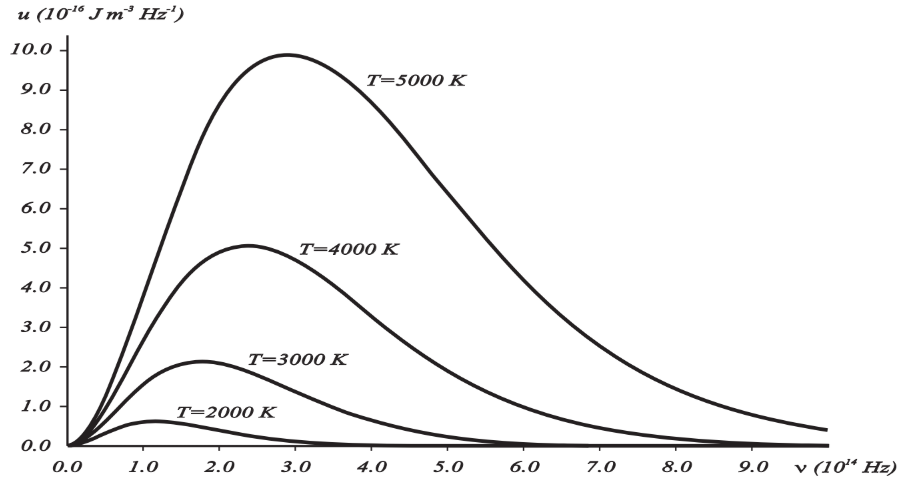
\includegraphics[width=0.5\textwidth]{Images/BlackBody.png}\label{fig:f1}}
        \caption{Spectral energy density of blackbody radiation at different temperatures as a function of the frequency}
    \end{figure}

    In 1879 J. Stefan found experimentally that the total intensity (or the total power per unit surface area) radiated by a glowing object of temperature $T$ is given by

    \begin{equation} \label{eq:1}
        \mathcal{P}=a \sigma T^{4} 
    \end{equation}

    \begin{figure}[H]
        \centering
        \subfloat[Blackbody Radiation Theories]{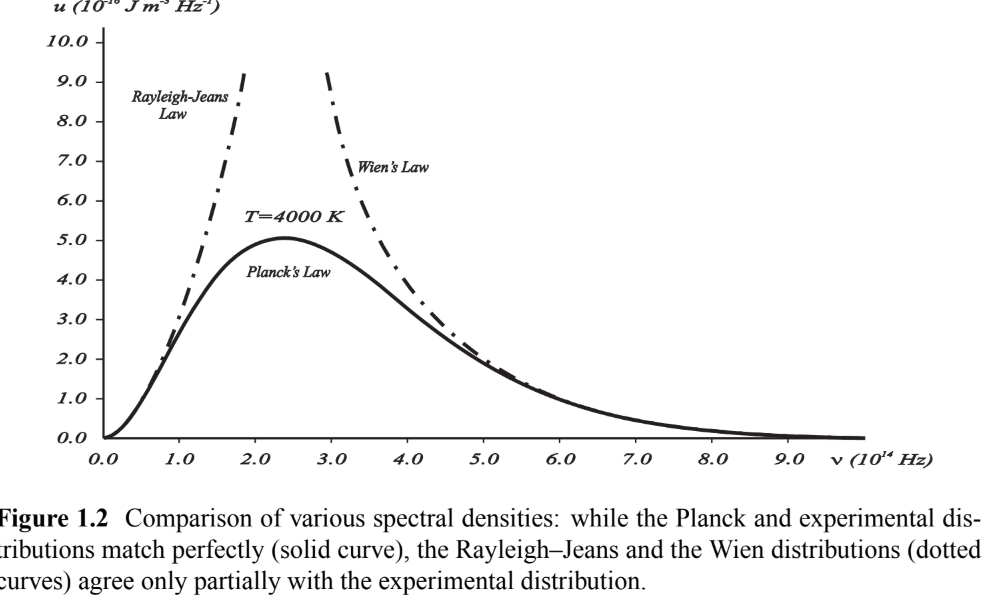
\includegraphics[width=0.5\textwidth]{Images/BlackbodyVSReal.png}\label{fig:f2}}
        \caption{Comparison of various spectral densities: while the Planck and experimental distributions match perfectly (solid curve), the Rayleigh-Jeans and the Wien distributions (dotted curves) agree only partially with the experimental distribution.}
    \end{figure}

    Wien took the Stefan-Boltzmann law equation \ref{eq:1} and in 1894 he extended it to obtain the energy density per unit frequency of the emitted blackbody radiation:

    \begin{equation} \label{eq:2}
        u(\nu, T)=A \nu^{3} e^{-\beta \nu / T} 
    \end{equation}

    Wien's formula fits the high-frequency data remarkably well, it fails badly at low frequencies (See figure \ref{fig:f2}.

    In his 1900 attempt, Rayleigh considered the radiation to consist of standing waves having a temperature $T$ with nodes at the metallic surfaces. These standing waves, he argued, are equivalent to harmonic oscillators from $\nu$ to $\nu+d \nu$ :

    \begin{equation} \label{eq:3}
        N(\nu)=\frac{8 \pi v^{2}}{c^{3}} 
    \end{equation}

    \begin{equation} \label{eq:4}
        u(\nu, T)=N(\nu)\langle E\rangle=\frac{8 \pi \nu^{2}}{c^{3}}\langle E\rangle 
    \end{equation}

    \begin{equation} \label{eq:5}
        \langle E\rangle=\frac{\int_{0}^{\infty} E e^{-E / k T} d E}{\int_{0}^{\infty} e^{-E / k T} d E}=k T 
    \end{equation}

    \begin{equation} \label{eq:6}
        u(\nu, T)=\frac{8 \pi \nu^{2}}{c^{3}} k T 
    \end{equation}


    Reayleigh-Jeans formula fits the low-frequency data remarkably well, it fails badly at high frequencies (See figure \ref{fig:f2}
     
    Planck succeeded in 1900 proposed an accurate description of blackbody radiation. Planck considered that the energy exchange between radiation and matter must be discrete. 

    \begin{equation} \label{eq:7}
        E =n h \nu 
    \end{equation}

    Assuming that the energy of an oscillator is quantized, replace the integration of equation \ref{eq:5} with a sum

    \begin{equation} \label{eq:8}
        \langle E\rangle=\frac{\sum_{n=0}^{\infty} n h \nu e^{-n h \nu / k T}}{\sum_{n=0}^{\infty} e^{-n h \nu / k T}}=\frac{h \nu}{e^{h \nu / k T}-1} 
    \end{equation}

    Plug into equation \ref{eq:4}

    \begin{equation} \label{eq:9}
        u(\nu, T)=\frac{8 \pi \nu^{2}}{c^{3}} \frac{h \nu}{e^{h \nu / k T}-1} 
    \end{equation}

    Using the conversion between wave frequency and wave length ($\lambda = \frac{c}{\nu}$

    \begin{equation} \label{eq:10}
        \tilde{u}(\lambda, T)=\frac{8 \pi h c}{\lambda^{5}} \frac{1}{e^{h c / \lambda k T}-1} 
    \end{equation}

    In the case of very low frequencies $h \nu \ll k T$, we can show that equation \ref{eq:9} reduces to the Rayleigh-Jeans law (equation \ref{eq:6}). Moreover, if we integrate Planck's distribution over the whole spectrum, we obtain the total energy density which is expressed in terms of Stefan-Boltzmann's total power per unit surface area as follows:

    Use the following change of variable
    \begin{equation} \label{eq:10.1}
        x=h \nu / k T
    \end{equation}

    Make use of the following special integral
    \begin{equation} \label{eq:10.2}
        \int_0^{\infty} \frac{x^3}{e^x - 1} dx = \frac{\pi^4}{15}
    \end{equation}
    
    \begin{equation} \label{eq:11}
    \int_{0}^{\infty} u(\nu, T) d \nu=\frac{8 \pi h}{c^{3}} \int_{0}^{\infty} \frac{\nu^{3}}{e^{h \nu / k T}-1} d \nu=\frac{8 \pi k^{4} T^{4}}{h^{3} c^{3}} \int_{0}^{\infty} \frac{x^{3}}{e^{x}-1} d x=\frac{8 \pi^{5} k^{4}}{15 h^{3} c^{3}} T^{4}=\frac{4}{c} \sigma T^{4} 
    \end{equation}

    In the limit of high frequencies, we can easily ascertain that Planck's distribution \ref{eq:9} yields Wien's rule \ref{eq:6}.

\subsection*{1.2.2 Photoelectric Effect}
    The photoelectric effect provides a direct confirmation for the energy quantization of light. In 1887 Hertz discovered the photoelectric effect, In 1899 J.J. Thomson confirmed that the particles giving rise to the photoelectric effect, the following experimental laws were discovered prior to 1905:

    \begin{itemize}
      \item If the frequency of the incident radiation is smaller than the metal's threshold no electron can be emitted regardless of the radiation's intensity (Philip Lenard, 1902).\textcolor{red}{Find this paper, put in bib}
      \item No matter how low the intensity of the incident radiation, electrons will be ejected instantly the moment the frequency of the radiation exceeds the threshold frequency $\nu_{0}$.
      \item At any frequency above $v_{0}$, the number of electrons ejected increases with the intensity of the light but does not depend on the light's frequency.
      \item The kinetic energy of the ejected electrons depends on the frequency but not on the intensity of the beam; the kinetic energy of the ejected electron increases linearly with the incident frequency.
    \end{itemize}

    According to classical physics, any (continuous) amount of energy can be exchanged with matter (i.e. any frequency with sufficient intensity can supply the necessary energy to free the electron from the metal)

    Einstein succeeded in 1905, He assumed that light is made of corpuscles each carrying an energy $h v$, called photons. 

    \begin{equation} \label{eq:12}
        h v=W_f+K_e 
    \end{equation}

    \begin{equation} \label{eq:13}
        K=h \nu-W=h\left(\nu-\nu_0\right) 
    \end{equation}

    \begin{equation}
        \nu_0 = \frac{W}{h}
    \end{equation}

    Upon experiment, the stopping potential depends linearly on the frequency of the incident radiation

    \begin{equation} \label{eq:14}
        V_{S}=\frac{h}{e} \nu-\frac{W}{e}=\frac{h c}{e \lambda}-\frac{W}{e} 
    \end{equation}

    Millikan who, in 1916, gave a systematic experimental confirmation to Einstein's photoelectric theory and obtained confirmation that $h$ is equal to Planck's constant to within a $0.5 \%$ experimental error.

\subsection*{1.2.3 Compton Effect}
    In 1923, Compton provided the most conclusive confirmation of the particle aspect of radiation by scattering X-rays off free electrons, he found that the wavelength of the scattered radiation is larger than the wavelength of the incident radiation. This can be explained only by assuming that the X-ray photons behave like particles.

    Consider that the incident photon, of energy $E=h v$ and momentum $p=h \nu / c$, collides with an electron that is initially at rest. If the photon scatters with a momentum $\overrightarrow{p^{\prime}}$ at an angle ${ }^{8}$ $\theta$ while the electron recoils with a momentum $\vec{P}_{e}$, the conservation of linear momentum yields


\begin{equation*}
\vec{p}=\vec{P}_{e}+\vec{p}^{\prime} \tag{1.28}
\end{equation*}


which leads to


\begin{equation*}
\vec{P}_{e}^{2}=\left(\vec{p}-\vec{p}^{\prime}\right)^{2}=p^{2}+p^{\prime 2}-2 p p^{\prime} \cos \theta=\frac{h^{2}}{c^{2}}\left(v^{2}+v^{\prime 2}-2 v v^{\prime} \cos \theta\right) \tag{1.29}
\end{equation*}


Let us now turn to the energy conservation. The energies of the electron before and after the collision are given, respectively, by


\begin{gather*}
E_{0}=m_{e} c^{2}  \tag{1.30}\\
E_{e}=\sqrt{\vec{P}_{e}^{2} c^{2}+m_{e}^{2} c^{4}}=h \sqrt{v^{2}+v^{\prime 2}-2 v v^{\prime} \cos \theta+\frac{m_{e}^{2} c^{4}}{h^{2}}} \tag{1.31}
\end{gather*}


in deriving this relation, we have used (1.29). Since the energies of the incident and scattered photons are given by $E=h \nu$ and $E^{\prime}=h \nu^{\prime}$, respectively, conservation of energy dictates that


\begin{equation*}
E+E_{0}=E^{\prime}+E_{e} \tag{1.32}
\end{equation*}


\footnotetext{${ }^{7}$ When a metal is irradiated with high energy radiation, and at sufficiently high frequencies-as in the case of X-rays-so that $h v$ is much larger than the binding energies of the electrons in the metal, these electrons can be considered as free.\\
${ }^{8}$ Here $\theta$ is the angle between $\vec{p}$ and $\vec{p}^{\prime}$, the photons' momenta before and after collision.
}
or\\
\$\$

\begin{equation*}
h v+m_{e} c^{2}=h v^{\prime}+h \sqrt{v^{2}+v^{\prime 2}-2 v v^{\prime} \cos \theta+\frac{m_{e}^{2} c^{4}}{h^{2}}}, \tag{1.33}
\end{equation*}

$$
which in turn leads to
$$

\begin{equation*}
v-v^{\prime}+\frac{m_{e} c^{2}}{h}=\sqrt{v^{2}+v^{\prime 2}-2 v v^{\prime} \cos \theta+\frac{m_{e}^{2} c^{4}}{h^{2}}} \tag{1.34}
\end{equation*}

\$\$

Squaring both sides of (1.34) and simplifying, we end up with


\begin{equation*}
\frac{1}{v^{\prime}}-\frac{1}{v}=\frac{h}{m_{e} c^{2}}(1-\cos \theta)=\frac{2 h}{m_{e} c^{2}} \sin ^{2}\left(\frac{\theta}{2}\right) \tag{1.35}
\end{equation*}


Hence the wavelength shift is given by


\begin{equation*}
\Delta \lambda=\lambda^{\prime}-\lambda=\frac{h}{m_{e} c}(1-\cos \theta)=2 \lambda_{C} \sin ^{2}\left(\frac{\theta}{2}\right) \tag{1.36}
\end{equation*}


where $\lambda_{C}=h /\left(m_{e} c\right)=2.426 \times 10^{-12} \mathrm{~m}$ is called the Compton wavelength of the electron. This relation, which connects the initial and final wavelengths to the scattering angle, confirms Compton's experimental observation: the wavelength shift of the X-rays depends only on the angle at which they are scattered and not on the frequency (or wavelength) of the incident photons.

In summary, the Compton effect confirms that photons behave like particles: they collide with electrons like material particles.

\section*{Example 1.3 (Compton effect)}
High energy photons ( $\gamma$-rays) are scattered from electrons initially at rest. Assume the photons are backscatterred and their energies are much larger than the electron's rest-mass energy, $E \gg$ $m_{e} c^{2}$.\\
(a) Calculate the wavelength shift.\\
(b) Show that the energy of the scattered photons is half the rest mass energy of the electron, regardless of the energy of the incident photons.\\
(c) Calculate the electron's recoil kinetic energy if the energy of the incident photons is 150 MeV .

\section*{Solution}
(a) In the case where the photons backscatter (i.e., $\theta=\pi$ ), the wavelength shift (1.36) becomes


\begin{equation*}
\Delta \lambda=\lambda^{\prime}-\lambda=2 \lambda_{C} \sin ^{2}\left(\frac{\pi}{2}\right)=2 \lambda_{C}=4.86 \times 10^{-12} \mathrm{~m} \tag{1.37}
\end{equation*}


since $\lambda_{C}=h /\left(m_{e} c\right)=2.426 \times 10^{-12} \mathrm{~m}$.\\
(b) Since the energy of the scattered photons $E^{\prime}$ is related to the wavelength $\lambda^{\prime}$ by $E^{\prime}=$ $h c / \lambda^{\prime}$, equation (1.37) yields


\begin{equation*}
E^{\prime}=\frac{h c}{\lambda^{\prime}}=\frac{h c}{\lambda+2 h /\left(m_{e} c\right)}=\frac{m_{e} c^{2}}{m_{e} c^{2} \lambda /(h c)+2}=\frac{m_{e} c^{2}}{m_{e} c^{2} / E+2} \tag{1.38}
\end{equation*}


\begin{center}
\includegraphics[max width=\textwidth]{2025_01_21_ba655ba27dcc3ebe44ebg-033}
\end{center}

Figure 1.5 Pair production: a highly energetic photon, interacting with a nucleus, disappears and produces an electron and a positron.\\
where $E=h c / \lambda$ is the energy of the incident photons. If $E \gg m_{e} c^{2}$ we can approximate (1.38) by


\begin{equation*}
E^{\prime}=\frac{m_{e} c^{2}}{2}\left[1+\frac{m_{e} c^{2}}{2 E}\right]^{-1} \simeq \frac{m_{e} c^{2}}{2}-\frac{\left(m_{e} c^{2}\right)^{2}}{4 E} \simeq \frac{m_{e} c^{2}}{2}=0.25 \mathrm{MeV} \tag{1.39}
\end{equation*}


(c) If $E=150 \mathrm{MeV}$, the kinetic energy of the recoiling electrons can be obtained from conservation of energy


\begin{equation*}
K_{e}=E-E^{\prime} \simeq 150 \mathrm{MeV}-0.25 \mathrm{MeV}=149.75 \mathrm{MeV} \tag{1.40}
\end{equation*}


\subsection*{1.2.4 Pair Production}
We deal here with another physical process which confirms that radiation (the photon) has corpuscular properties.

The theory of quantum mechanics that Schrödinger and Heisenberg proposed works only for nonrelativistic phenomena. This theory, which is called nonrelativistic quantum mechanics, was immensely successful in explaining a wide range of such phenomena. Combining the theory of special relativity with quantum mechanics, Dirac succeeded (1928) in extending quantum mechanics to the realm of relativistic phenomena. The new theory, called relativistic quantum mechanics, predicted the existence of a new particle, the positron. This particle, defined as the antiparticle of the electron, was predicted to have the same mass as the electron and an equal but opposite (positive) charge.

Four years after its prediction by Dirac's relativistic quantum mechanics, the positron was discovered by Anderson in 1932 while studying the trails left by cosmic rays in a cloud chamber. When high-frequency electromagnetic radiation passes through a foil, individual photons of this radiation disappear by producing a pair of particles consisting of an electron, $e^{-}$, and a positron, $e^{+}$: photon $\rightarrow e^{-}+e^{+}$. This process is called pair production; Anderson obtained such a process by exposing a lead foil to cosmic rays from outer space which contained highly energetic X-rays. It is useless to attempt to explain the pair production phenomenon by means of classical physics, because even nonrelativistic quantum mechanics fails utterly to account for $i t$.

Due to charge, momentum, and energy conservation, pair production cannot occur in empty space. For the process photon $\rightarrow e^{-}+e^{+}$to occur, the photon must interact with an external field such as the Coulomb field of an atomic nucleus to absorb some of its momentum. In the\\
reaction depicted in Figure 1.5, an electron-positron pair is produced when the photon comes near (interacts with) a nucleus at rest; energy conservation dictates that


\begin{align*}
\hbar \omega & =E_{e^{-}}+E_{e^{+}}+E_{N}=\left(m_{e} c^{2}+k_{e^{-}}\right)+\left(m_{e} c^{2}+k_{e^{+}}\right)+K_{N} \\
& \simeq 2 m_{e} c^{2}+k_{e^{-}}+k_{e^{+}} \tag{1.41}
\end{align*}


where $\hbar \omega$ is the energy of the incident photon, $2 m_{e} c^{2}$ is the sum of the rest masses of the electron and positron, and $k_{e^{-}}$and $k_{e^{+}}$are the kinetic energies of the electron and positron, respectively. As for $E_{N}=K_{N}$, it represents the recoil energy of the nucleus which is purely kinetic. Since the nucleus is very massive compared to the electron and the positron, $K_{N}$ can be neglected to a good approximation. Note that the photon cannot produce an electron or a positron alone, for electric charge would not be conserved. Also, a massive object, such as the nucleus, must participate in the process to take away some of the photon's momentum.

The inverse of pair production, called pair annihilation, also occurs. For instance, when an electron and a positron collide, they annihilate each other and give rise to electromagnetic radiation ${ }^{9}: e^{-}+e^{+} \rightarrow$ photon. This process explains why positrons do not last long in nature. When a positron is generated in a pair production process, its passage through matter will make it lose some of its energy and it eventually gets annihilated after colliding with an electron. The collision of a positron with an electron produces a hydrogen-like atom, called positronium, with a mean lifetime of about $10^{-10} \mathrm{~s}$; positronium is like the hydrogen atom where the proton is replaced by the positron. Note that, unlike pair production, energy and momentum can simultaneously be conserved in pair annihilation processes without any additional (external) field or mass such as the nucleus.

The pair production process is a direct consequence of the mass-energy equation of Einstein $E=m c^{2}$, which states that pure energy can be converted into mass and vice versa. Conversely, pair annihilation occurs as a result of mass being converted into pure energy. All subatomic particles also have antiparticles (e.g., antiproton). Even neutral particles have antiparticles; for instance, the antineutron is the neutron's antiparticle. Although this text deals only with nonrelativistic quantum mechanics, we have included pair production and pair annihilation, which are relativistic processes, merely to illustrate how radiation interacts with matter, and also to underscore the fact that the quantum theory of Schrödinger and Heisenberg is limited to nonrelativistic phenomena only.

\section*{Example 1.4 (Minimum energy for pair production)}
Calculate the minimum energy of a photon so that it converts into an electron-positron pair. Find the photon's frequency and wavelength.

\section*{Solution}
The minimum energy $E_{\min }$ of a photon required to produce an electron-positron pair must be equal to the sum of rest mass energies of the electron and positron; this corresponds to the case where the kinetic energies of the electron and positron are zero. Equation (1.41) yields


\begin{equation*}
E_{\min }=2 m_{e} c^{2}=2 \times 0.511 \mathrm{MeV}=1.02 \mathrm{MeV} \tag{1.42}
\end{equation*}


\footnotetext{${ }^{9}$ When an electron-positron pair annihilate, they produce at least two photons each having an energy $m_{e} c^{2}=$ 0.511 MeV .
}If the photon's energy is smaller than 1.02 MeV , no pair will be produced. The photon's frequency and wavelength can be obtained at once from $E_{\text {min }}=h \nu=2 m_{e} c^{2}$ and $\lambda=c / \nu$ :


\begin{gather*}
v=\frac{2 m_{e} c^{2}}{h}=\frac{2 \times 9.1 \times 10^{-31} \mathrm{~kg} \times\left(3 \times 10^{8} \mathrm{~m} \mathrm{~s}^{-1}\right)^{2}}{6.63 \times 10^{-34} \mathrm{~J} \mathrm{~s}}=2.47 \times 10^{20} \mathrm{~Hz}  \tag{1.43}\\
\lambda=\frac{c}{v}=\frac{3 \times 10^{8} \mathrm{~m} \mathrm{~s}^{-1}}{2.47 \times 10^{20} \mathrm{~Hz}}=1.2 \times 10^{-12} \mathrm{~m} \tag{1.44}
\end{gather*}


\subsection*{1.3 Wave Aspect of Particles}
\subsection*{1.3.1 de Broglie's Hypothesis: Matter Waves}
As discussed above-in the photoelectric effect, the Compton effect, and the pair production effect-radiation exhibits particle-like characteristics in addition to its wave nature. In 1923 de Broglie took things even further by suggesting that this wave-particle duality is not restricted to radiation, but must be universal: all material particles should also display a dual wave-particle behavior. That is, the wave-particle duality present in light must also occur in matter.

So, starting from the momentum of a photon $p=h \nu / c=h / \lambda$, we can generalize this relation to any material particle ${ }^{10}$ with nonzero rest mass: each material particle of momentum $\vec{p}$ behaves as a group of waves (matter waves) whose wavelength $\lambda$ and wave vector $\vec{k}$ are governed by the speed and mass of the particle


\begin{equation*}
\lambda=\frac{h}{p}, \quad \vec{k}=\frac{\vec{p}}{\hbar} \tag{1.45}
\end{equation*}


where $\hbar=h / 2 \pi$. The expression (1.45), known as the de Broglie relation, connects the momentum of a particle with the wavelength and wave vector of the wave corresponding to this particle.

\subsection*{1.3.2 Experimental Confirmation of de Broglie's Hypothesis}
de Broglie's idea was confirmed experimentally in 1927 by Davisson and Germer, and later by Thomson, who obtained interference patterns with electrons.

\subsection*{1.3.2.1 Davisson-Germer Experiment}
In their experiment, Davisson and Germer scattered a 54 eV monoenergetic beam of electrons from a nickel $(\mathrm{Ni})$ crystal. The electron source and detector were symmetrically located with respect to the crystal's normal, as indicated in Figure 1.6; this is similar to the Bragg setup for X-ray diffraction by a grating. What Davisson and Germer found was that, although the electrons are scattered in all directions from the crystal, the intensity was a minimum at $\theta=35^{\circ}$

\footnotetext{${ }^{10}$ In classical physics a particle is characterized by its energy $E$ and its momentum $\vec{p}$, whereas a wave is characterized by its wavelength $\lambda$ and its wave vector $\vec{k}=(2 \pi / \lambda) \hat{n}$, where $\hat{n}$ is a unit vector that specifies the direction of propagation of the wave.
}
\includegraphics[max width=\textwidth, center]{2025_01_21_ba655ba27dcc3ebe44ebg-036}

Figure 1.6 Davisson-Germer experiment: electrons strike the crystal's surface at an angle $\phi$; the detector, symmetrically located from the electron source, measures the number of electrons scattered at an angle $\theta$, where $\theta$ is the angle between the incident and scattered electron beams.\\
and a maximum at $\theta=50^{\circ}$; that is, the bulk of the electrons scatter only in well-specified directions. They showed that the pattern persisted even when the intensity of the beam was so low that the incident electrons were sent one at a time. This can only result from a constructive interference of the scattered electrons. So, instead of the diffuse distribution pattern that results from material particles, the reflected electrons formed diffraction patterns that were identical with Bragg's X-ray diffraction by a grating. In fact, the intensity maximum of the scattered electrons in the Davisson-Germer experiment corresponds to the first maximum ( $n=1$ ) of the Bragg formula,


\begin{equation*}
n \lambda=2 d \sin \phi \tag{1.46}
\end{equation*}


where $d$ is the spacing between the Bragg planes, $\phi$ is the angle between the incident ray and the crystal's reflecting planes, $\theta$ is the angle between the incident and scattered beams ( $d$ is given in terms of the separation $D$ between successive atomic layers in the crystal by $d=D \sin \theta$ ).

For an Ni crystal, we have $d=0.091 \mathrm{~nm}$, since $D=0.215 \mathrm{~nm}$. Since only one maximum is seen at $\theta=50^{\circ}$ for a mono-energetic beam of electrons of kinetic energy 54 eV , and since $2 \phi+\theta=\pi$ and hence $\sin \phi=\cos (\theta / 2)$ (Figure 1.6), we can obtain from (1.46) the wavelength associated with the scattered electrons:


\begin{equation*}
\lambda=\frac{2 d}{n} \sin \phi=\frac{2 d}{n} \cos \frac{1}{2} \theta=\frac{2 \times 0.091 \mathrm{~nm}}{1} \cos 25^{\circ}=0.165 \mathrm{~nm} \tag{1.47}
\end{equation*}


Now, let us look for the numerical value of $\lambda$ that results from de Broglie's relation. Since the kinetic energy of the electrons is $K=54 \mathrm{eV}$, and since the momentum is $p=\sqrt{2 m_{e} K}$ with $m_{e} c^{2}=0.511 \mathrm{MeV}$ (the rest mass energy of the electron) and $\hbar c \simeq 197.33 \mathrm{eV} \mathrm{nm}$, we can show that the de Broglie wavelength is


\begin{equation*}
\lambda=\frac{h}{p}=\frac{h}{\sqrt{2 m_{e} K}}=\frac{2 \pi \hbar c}{\sqrt{2 m_{e} c^{2} K}}=0.167 \mathrm{~nm} \tag{1.48}
\end{equation*}


which is in excellent agreement with the experimental value (1.47).\\
We have seen that the scattered electrons in the Davisson-Germer experiment produced interference fringes that were identical to those of Bragg's X-ray diffraction. Since the Bragg formula provided an accurate prediction of the electrons' interference fringes, the motion of an electron of momentum $\vec{p}$ must be described by means of a plane wave


\begin{equation*}
\psi(\vec{r}, t)=A e^{i(\vec{k} \cdot \vec{r}-\omega t)}=A e^{i(\vec{p} \cdot \vec{r}-E t) / \hbar} \tag{1.49}
\end{equation*}


\begin{center}
\includegraphics[max width=\textwidth]{2025_01_21_ba655ba27dcc3ebe44ebg-037}
\end{center}

Figure 1.7 Thomson experiment: diffraction of electrons through a thin film of polycrystalline material yields fringes that usually result from light diffraction.\\
where $A$ is a constant, $\vec{k}$ is the wave vector of the plane wave, and $\omega$ is its angular frequency; the wave's parameters, $\vec{k}$ and $\omega$, are related to the electron's momentum $\vec{p}$ and energy $E$ by means of de Broglie's relations: $\vec{k}=\vec{p} / \hbar, \omega=E / \hbar$.

We should note that, inspired by de Broglie's hypothesis, Schrödinger constructed the theory of wave mechanics which deals with the dynamics of microscopic particles. He described the motion of particles by means of a wave function $\psi(\vec{r}, t)$ which corresponds to the de Broglie wave of the particle. We will deal with the physical interpretation of $\psi(\vec{r}, t)$ in the following section.

\subsection*{1.3.2.2 Thomson Experiment}
In the Thomson experiment (Figure 1.7), electrons were diffracted through a polycrystalline thin film. Diffraction fringes were also observed. This result confirmed again the wave behavior of electrons.

The Davisson-Germer experiment has inspired others to obtain diffraction patterns with a large variety of particles. Interference patterns were obtained with bigger and bigger particles such as neutrons, protons, helium atoms, and hydrogen molecules. de Broglie wave interference of carbon 60 (C60) molecules were recently ${ }^{11}$ observed by diffraction at a material absorption grating; these observations supported the view that each C60 molecule interferes only with itself (a C60 molecule is nearly a classical object).

\subsection*{1.3.3 Matter Waves for Macroscopic Objects}
We have seen that microscopic particles, such as electrons, display wave behavior. What about macroscopic objects? Do they also display wave features? They surely do. Although macro-

\footnotetext{${ }^{11}$ Markus Arndt, et al., "Wave-Particle Duality of C60 Molecules", Nature, V401, n6754, 680 (Oct. 14, 1999).
}
scopic material particles display wave properties, the corresponding wavelengths are too small to detect; being very massive ${ }^{12}$, macroscopic objects have extremely small wavelengths. At the microscopic level, however, the waves associated with material particles are of the same size or exceed the size of the system. Microscopic particles therefore exhibit clearly discernible wave-like aspects.

The general rule is: whenever the de Broglie wavelength of an object is in the range of, or exceeds, its size, the wave nature of the object is detectable and hence cannot be neglected. But if its de Broglie wavelength is much too small compared to its size, the wave behavior of this object is undetectable. For a quantitative illustration of this general rule, let us calculate in the following example the wavelengths corresponding to two particles, one microscopic and the other macroscopic.

\section*{Example 1.5 (Matter waves for microscopic and macroscopic systems)}
Calculate the de Broglie wavelength for\\
(a) a proton of kinetic energy 70 MeV kinetic energy and\\
(b) a 100 g bullet moving at $900 \mathrm{~m} \mathrm{~s}^{-1}$.

\section*{Solution}
(a) Since the kinetic energy of the proton is $T=p^{2} /\left(2 m_{p}\right)$, its momentum is $p=\sqrt{2 T m_{p}}$. The de Broglie wavelength is $\lambda_{p}=h / p=h / \sqrt{2 T_{p}}$. To calculate this quantity numerically, it is more efficient to introduce the well-known quantity $\hbar c \simeq 197 \mathrm{MeV} \mathrm{fm}$ and the rest mass of the proton $m_{p} c^{2}=938.3 \mathrm{MeV}$, where $c$ is the speed of light:


\begin{equation*}
\lambda_{p}=2 \pi \frac{\hbar c}{p c}=2 \pi \frac{\hbar c}{\sqrt{2 T m_{p} c^{2}}}=2 \pi \frac{197 \mathrm{MeV} \mathrm{fm}}{\sqrt{2 \times 938.3 \times 70 \mathrm{MeV}^{2}}}=3.4 \times 10^{-15} \mathrm{~m} \tag{1.50}
\end{equation*}


(b) As for the bullet, its de Broglie wavelength is $\lambda_{b}=h / p=h /(m v)$ and since $h=$ $6.626 \times 10^{-34} \mathrm{~J} \mathrm{~s}$, we have


\begin{equation*}
\lambda_{b}=\frac{h}{m v}=\frac{6.626 \times 10^{-34} \mathrm{~J} \mathrm{~s}}{0.1 \mathrm{~kg} \times 900 \mathrm{~m} \mathrm{~s}^{-1}}=7.4 \times 10^{-36} \mathrm{~m} \tag{1.51}
\end{equation*}


The ratio of the two wavelengths is $\lambda_{b} / \lambda_{p} \simeq 2.2 \times 10^{-21}$. Clearly, the wave aspect of this bullet lies beyond human observational abilities. As for the wave aspect of the proton, it cannot be neglected; its de Broglie wavelength of $3.4 \times 10^{-15} \mathrm{~m}$ has the same order of magnitude as the size of a typical atomic nucleus.

We may conclude that, whereas the wavelengths associated with microscopic systems are finite and display easily detectable wave-like patterns, the wavelengths associated with macroscopic systems are infinitesimally small and display no discernible wave-like behavior. So, when the wavelength approaches zero, the wave-like properties of the system disappear. In such cases of infinitesimally small wavelengths, geometrical optics should be used to describe the motion of the object, for the wave associated with it behaves as a ray.

\footnotetext{${ }^{12}$ Very massive compared to microscopic particles. For instance, the ratio between the mass of an electron and a 100 g bullet is infinitesimal: $m_{e} / m_{b} \simeq 10^{-29}$.
}
\includegraphics[max width=\textwidth, center]{2025_01_21_ba655ba27dcc3ebe44ebg-039}

Figure 1.8 The double-slit experiment with particles: $S$ is a source of bullets; $I_{1}$ and $I_{2}$ are the intensities recorded on the screen, respectively, when only $S_{1}$ is open and then when only $S_{2}$ is open. When both slits are open, the total intensity is $I=I_{1}+I_{2}$.

\subsection*{1.4 Particles versus Waves}
In this section we are going to study the properties of particles and waves within the contexts of classical and quantum physics. The experimental setup to study these aspects is the double-slit experiment, which consists of a source $S$ ( $S$ can be a source of material particles or of waves), a wall with two slits $S_{1}$ and $S_{2}$, and a back screen equipped with counters that record whatever arrives at it from the slits.

\subsection*{1.4.1 Classical View of Particles and Waves}
In classical physics, particles and waves are mutually exclusive; they exhibit completely different behaviors. While the full description of a particle requires only one parameter, the position vector $\vec{r}(t)$, the complete description of a wave requires two, the amplitude and the phase. For instance, three-dimensional plane waves can be described by wave functions $\psi(\vec{r}, t)$ :


\begin{equation*}
\psi(\vec{r}, t)=A e^{i(\vec{k} \cdot \vec{r}-\omega t)}=A e^{i \phi} \tag{1.52}
\end{equation*}


where $A$ is the amplitude of the wave and $\phi$ is its phase $(\vec{k}$ is the wave vector and $\omega$ is the angular frequency). We may recall the physical meaning of $\psi$ : the intensity of the wave is given by $I=|\psi|^{2}$.

\section*{(a) $S$ is a source of streams of bullets}
Consider three different experiments as displayed in Figure 1.8, in which a source $S$ fires a stream of bullets; the bullets are assumed to be indestructible and hence arrive on the screen in identical lumps. In the first experiment, only slit $S_{1}$ is open; let $I_{1}(y)$ be the corresponding intensity collected on the screen (the number of bullets arriving per second at a given point $y$ ). In the second experiment, let $I_{2}(y)$ be the intensity collected on the screen when only $S_{2}$ is open. In the third experiments, if $S_{1}$ and $S_{2}$ are both open, the total intensity collected on the\\
\includegraphics[max width=\textwidth, center]{2025_01_21_ba655ba27dcc3ebe44ebg-040}

Figure 1.9 The double-slit experiment: $S$ is a source of waves, $I_{1}$ and $I_{2}$ are the intensities recorded on the screen when only $S_{1}$ is open, and then when only $S_{2}$ is open, respectively. When both slits are open, the total intensity is no longer equal to the sum of $I_{1}$ and $I_{2}$; an oscillating term has to be added.\\
screen behind the two slits must be equal to the sum of $I_{1}$ and $I_{2}$ :


\begin{equation*}
I(y)=I_{1}(y)+I_{2}(y) \tag{1.53}
\end{equation*}


\section*{(b) $S$ is a source of waves}
Now, as depicted in Figure 1.9, $S$ is a source of waves (e.g., light or water waves). Let $I_{1}$ be the intensity collected on the screen when only $S_{1}$ is open and $I_{2}$ be the intensity when only $S_{2}$ is open. Recall that a wave is represented by a complex function $\psi$, and its intensity is proportional to its amplitude (e.g., height of water or electric field) squared: $I_{1}=\left|\psi_{1}\right|^{2}, I_{2}=\left|\psi_{2}\right|^{2}$. When both slits are open, the total intensity collected on the screen displays an interference pattern; hence it cannot be equal to the sum of $I_{1}$ and $I_{2}$. The amplitudes, not the intensities, must add: the total amplitude $\psi$ is the sum of $\psi_{1}$ and $\psi_{2}$; hence the total intensity is given by


\begin{align*}
I=\left|\psi_{1}+\psi_{2}\right|^{2} & =\left|\psi_{1}\right|^{2}+\left|\psi_{2}\right|^{2}+\left(\psi_{1}^{*} \psi_{2}+\psi_{2}^{*} \psi_{1}\right)=I_{1}+I_{2}+2 \operatorname{Re}\left(\psi_{1}^{*} \psi_{2}\right) \\
& =I_{1}+I_{2}+2 \sqrt{I_{1} I_{2}} \cos \delta \tag{1.54}
\end{align*}


where $\delta$ is the phase difference between $\psi_{1}$ and $\psi_{2}$, and $2 \sqrt{I_{1} I_{2}} \cos \delta$ is an oscillating term, which is responsible for the interference pattern (Figure 1.9). So the resulting intensity distribution cannot be predicted from $I_{1}$ or from $I_{2}$ alone, for it depends on the phase $\delta$, which cannot be measured when only one slit is open ( $\delta$ can be calculated from the slits separation or from the observed intensities $I_{1}, I_{2}$ and $I$ ).\\
Conclusion: Classically, waves exhibit interference patterns, particles do not. When two noninteracting streams of particles combine in the same region of space, their intensities add; when waves combine, their amplitudes add but their intensities do not.

\subsection*{1.4.2 Quantum View of Particles and Waves}
Let us now discuss the double-slit experiment with quantum material particles such as electrons. Figure 1.10 shows three different experiments where the source $S$ shoots a stream of electrons,\\
\includegraphics[max width=\textwidth, center]{2025_01_21_ba655ba27dcc3ebe44ebg-041}

Figure 1.10 The double-slit experiment: $S$ is a source of electrons, $I_{1}$ and $I_{2}$ are the intensities recorded on the screen when only $S_{1}$ is open, and then when only $S_{2}$ is open, respectively. When both slits are open, the total intensity is equal to the sum of $I_{1}, I_{2}$ and an oscillating term.\\
first with only $S_{1}$ open, then with only $S_{2}$ open, and finally with both slits open. In the first two cases, the distributions of the electrons on the screen are smooth; the sum of these distributions is also smooth, a bell-shaped curve like the one obtained for classical particles (Figure 1.8).

But when both slits are open, we see a rapid variation in the distribution, an interference pattern. So in spite of their discreteness, the electrons seem to interfere with themselves; this means that each electron seems to have gone through both slits at once! One might ask, if an electron cannot be split, how can it appear to go through both slits at once? Note that this interference pattern has nothing to do with the intensity of the electron beam. In fact, experiments were carried out with beams so weak that the electrons were sent one at a time (i.e., each electron was sent only after the previous electron has reached the screen). In this case, if both slits were open and if we wait long enough so that sufficient impacts are collected on the screen, the interference pattern appears again.

The crucial question now is to find out the slit through which the electron went. To answer this query, an experiment can be performed to watch the electrons as they leave the slits. It consists of placing a strong light source behind the wall containing the slits, as shown in Figure 1.11. We place Geiger counters all over the screen so that whenever an electron reaches the screen we hear a click on the counter.

Since electric charges scatter light, whenever an electron passes through either of the slits, on its way to the counter, it will scatter light to our eyes. So, whenever we hear a click on the counter, we see a flash near either $S_{1}$ or $S_{2}$ but never near both at once. After recording the various counts with both slits open, we find out that the distribution is similar to that of classical bullets in Figure 1.8: the interference pattern has disappeared! But if we turn off the light source, the interference pattern appears again.

From this experiment we conclude that the mere act of looking at the electrons immensely affects their distribution on the screen. Clearly, electrons are very delicate: their motion gets modified when one watches them. This is the very quantum mechanical principle which states that measurements interfere with the states of microscopic objects. One might think of turning down the brightness (intensity) of the light source so that it is weak enough not to disturb the\\
\includegraphics[max width=\textwidth, center]{2025_01_21_ba655ba27dcc3ebe44ebg-042}

Figure 1.11 The double-slit experiment: $S$ is a source of electrons. A light source is placed behind the wall containing $S_{1}$ and $S_{2}$. When both slits are open, the interference pattern is destroyed and the total intensity is $I=I_{1}+I_{2}$.\\
electrons. We find that the light scattered from the electrons, as they pass by, does not get weaker; the same sized flash is seen, but only every once in a while. This means that, at low brightness levels, we miss some electrons: we hear the click from the counter but see no flash at all. At still lower brightness levels, we miss most of the electrons. We conclude, in this case, that some electrons went through the slits without being seen, because there were no photons around at the right moment to catch them. This process is important because it confirms that light has particle properties: light also arrives in lumps (photons) at the screen.

Two distribution profiles are compiled from this dim light source experiment, one corresponding to the electrons that were seen and the other to the electrons that were not seen (but heard on the counter). The first distribution contains no interference (i.e., it is similar to classical bullets); but the second distribution displays an interference pattern. This results from the fact that when the electrons are not seen, they display interference. When we do not see the electron, no photon has disturbed it but when we see it, a photon has disturbed it.

For the electrons that display interference, it is impossible to identify the slit that each electron had gone through. This experimental finding introduces a new fundamental concept: the microphysical world is indeterministic. Unlike classical physics, where we can follow accurately the particles along their trajectories, we cannot follow a microscopic particle along its motion nor can we determine its path. It is technically impossible to perform such detailed tracing of the particle's motion. Such results inspired Heisenberg to postulate the uncertainty principle, which states that it is impossible to design an apparatus which allows us to determine the slit that the electron went through without disturbing the electron enough to destroy the interference pattern (we shall return to this principle later).

The interference pattern obtained from the double-slit experiment indicates that electrons display both particle and wave properties. When electrons are observed or detected one by one, they behave like particles, but when they are detected after many measurements (distribution of the detected electrons), they behave like waves of wavelength $\lambda=h / p$ and display an interference pattern.

\subsection*{1.4.3 Wave-Particle Duality: Complementarity}
The various experimental findings discussed so far-blackbody radiation, photoelectric and Compton effect, pair production, Davisson-Germer, Thomson, and the double-slit experimentsreveal that photons, electrons, and any other microscopic particles behave unlike classical particles and unlike classical waves. These findings indicate that, at the microscopic scale, nature can display particle behavior as well as wave behavior. The question now is, how can something behave as a particle and as a wave at the same time? Aren't these notions mutually exclusive? In the realm of classical physics the answer is yes, but not in quantum mechanics. This dual behavior can in no way be reconciled within the context of classical physics, for particles and waves are mutually exclusive entities.

The theory of quantum mechanics, however, provides the proper framework for reconciling the particle and wave aspects of matter. By using a wave function $\psi(\vec{r}, t)$ (see (1.49)) to describe material particles such as electrons, quantum mechanics can simultaneously make statements about the particle behavior and the wave behavior of microscopic systems. It combines the quantization of energy or intensity with a wave description of matter. That is, it uses both particle and wave pictures to describe the same material particle.

Our ordinary concepts of particles or waves are thus inadequate when applied to microscopic systems. These two concepts, which preclude each other in the macroscopic realm, do not strictly apply to the microphysical world. No longer valid at the microscopic scale is the notion that a wave cannot behave as a particle and vice versa. The true reality of a quantum system is that it is neither a pure particle nor a pure wave. The particle and wave aspects of a quantum system manifest themselves only when subjected to, or intruded on by, penetrating means of observation (any procedure of penetrating observation would destroy the initial state of the quantum system; for instance, the mere act of looking at an electron will knock it out of its orbit). Depending on the type of equipment used to observe an electron, the electron has the capacity to display either "grain" or wave features. As illustrated by the double-slit experiment, if we wanted to look at the particle aspect of the electron, we would need only to block one slit (or leave both slits open but introduce an observational apparatus), but if we were interested only in its wave features, we would have to leave both slits open and not intrude on it by observational tools. This means that both the "grain" and "wave" features are embedded into the electron, and by modifying the probing tool, we can suppress one aspect of the electron and keep the other. An experiment designed to isolate the particle features of a quantum system gives no information about its wave features, and vice versa. When we subject an electron to Compton scattering, we observe only its particle aspects, but when we involve it in a diffraction experiment (as in Davisson-Germer, Thomson, or the double-slit experiment), we observe its wave behavior only. So if we measure the particle properties of a quantum system, this will destroy its wave properties, and vice versa. Any measurement gives either one property or the other, but never both at once. We can get either the wave property or the particle but not both of them together.

Microscopic systems, therefore, are neither pure particles nor pure waves, they are both. The particle and wave manifestations do not contradict or preclude one another, but, as suggested by Bohr, they are just complementary. Both concepts are complementary in describing the true nature of microscopic systems. Being complementary features of microscopic matter, particles and waves are equally important for a complete description of quantum systems. From here comes the essence of the complementarity principle.

We have seen that when the rigid concept of either/or (i.e., either a particle or a wave) is indiscriminately applied or imposed on quantum systems, we get into trouble with reality.

Without the complementarity principle, quantum mechanics would not have been in a position to produce the accurate results it does.

\subsection*{1.4.4 Principle of Linear Superposition}
How do we account mathematically for the existence of the interference pattern in the doubleslit experiment with material particles such as electrons? An answer is offered by the superposition principle. The interference results from the superposition of the waves emitted by slits 1 and 2. If the functions $\psi_{1}(\vec{r}, t)$ and $\psi_{2}(\vec{r}, t)$, which denote the waves reaching the screen emitted respectively by slits 1 and 2 , represent two physically possible states of the system, then any linear superposition


\begin{equation*}
\psi(\vec{r}, t)=\alpha_{1} \psi_{1}(\vec{r}, t)+\alpha_{2} \psi_{2}(\vec{r}, t) \tag{1.55}
\end{equation*}


also represents a physically possible outcome of the system; $\alpha_{1}$ and $\alpha_{2}$ are complex constants. This is the superposition principle. The intensity produced on the screen by opening only slit 1 is $\left|\psi_{1}(\vec{r}, t)\right|^{2}$ and it is $\left|\psi_{2}(\vec{r}, t)\right|^{2}$ when only slit 2 is open. When both slits are open, the intensity is


\begin{align*}
|\psi(\vec{r}, t)|^{2} & =\left|\psi_{1}(\vec{r}, t)+\psi_{2}(\vec{r}, t)\right|^{2} \\
& =\left|\psi_{1}(\vec{r}, t)\right|^{2}+\left|\psi_{2}(\vec{r}, t)\right|^{2}+\psi_{1}^{*}(\vec{r}, t) \psi_{2}(\vec{r}, t)+\psi_{1}(\vec{r}, t) \psi_{2}^{*}(\vec{r}, t) \tag{1.56}
\end{align*}


where the asterisk denotes the complex conjugate. Note that (1.56) is not equal to the sum of $\left|\psi_{1}(\vec{r}, t)\right|^{2}$ and $\left|\psi_{2}(\vec{r}, t)\right|^{2}$; it contains an additional term $\psi_{1}^{*}(\vec{r}, t) \psi_{2}(\vec{r}, t)+\psi_{1}(\vec{r}, t) \psi_{2}^{*}(\vec{r}, t)$. This is the very term which gives rise in the case of electrons to an interference pattern similar to light waves. The interference pattern therefore results from the existence of a phase shift between $\psi_{1}(\vec{r}, t)$ and $\psi_{2}(\vec{r}, t)$. We can measure this phase shift from the interference pattern, but we can in no way measure the phases of $\psi_{1}$ and $\psi_{2}$ separately.

We can summarize the double-slit results in three principles:

\begin{itemize}
  \item Intensities add for classical particles: $I=I_{1}+I_{2}$.
  \item Amplitudes, not intensities, add for quantum particles: $\psi(\vec{r}, t)=\psi_{1}(\vec{r}, t)+\psi_{2}(\vec{r}, t)$; this gives rise to interference.
  \item Whenever one attempts to determine experimentally the outcome of individual events for microscopic material particles (such as trying to specify the slit through which an electron has gone), the interference pattern gets destroyed. In this case the intensities add in much the same way as for classical particles: $I=I_{1}+I_{2}$.
\end{itemize}

\subsection*{1.5 Indeterministic Nature of the Microphysical World}
Let us first mention two important experimental findings that were outlined above. On the one hand, the Davisson-Germer and the double-slit experiments have shown that microscopic material particles do give rise to interference patterns. To account for the interference pattern, we have seen that it is imperative to describe microscopic particles by means of waves. Waves are\\
not localized in space. As a result, we have to give up on accuracy to describe microscopic particles, for waves give at best a probabilistic account. On the other hand, we have seen in the double-slit experiment that it is impossible to trace the motion of individual electrons; there is no experimental device that would determine the slit through which a given electron has gone. Not being able to predict single events is a stark violation of a founding principle of classical physics: predictability or determinacy. These experimental findings inspired Heisenberg to postulate the indeterministic nature of the microphysical world and Born to introduce the probabilistic interpretation of quantum mechanics.

\subsection*{1.5.1 Heisenberg's Uncertainty Principle}
According to classical physics, given the initial conditions and the forces acting on a system, the future behavior (unique path) of this physical system can be determined exactly. That is, if the initial coordinates $\vec{r}_{0}$, velocity $\vec{v}_{0}$, and all the forces acting on the particle are known, the position $\vec{r}(t)$ and velocity $\vec{v}(t)$ are uniquely determined by means of Newton's second law. Classical physics is thus completely deterministic.

Does this deterministic view hold also for the microphysical world? Since a particle is represented within the context of quantum mechanics by means of a wave function corresponding to the particle's wave, and since wave functions cannot be localized, then a microscopic particle is somewhat spread over space and, unlike classical particles, cannot be localized in space. In addition, we have seen in the double-slit experiment that it is impossible to determine the slit that the electron went through without disturbing it. The classical concepts of exact position, exact momentum, and unique path of a particle therefore make no sense at the microscopic scale. This is the essence of Heisenberg's uncertainty principle.

In its original form, Heisenberg's uncertainty principle states that: If the $x$-component of the momentum of a particle is measured with an uncertainty $\Delta p_{x}$, then its $x$-position cannot, at the same time, be measured more accurately than $\Delta x=\hbar /\left(2 \Delta p_{x}\right)$. The three-dimensional form of the uncertainty relations for position and momentum can be written as follows:


\begin{equation*}
\Delta x \Delta p_{x} \geq \frac{\hbar}{2}, \quad \Delta y \Delta p_{y} \geq \frac{\hbar}{2}, \quad \Delta z \Delta p_{z} \geq \frac{\hbar}{2} \tag{1.57}
\end{equation*}


This principle indicates that, although it is possible to measure the momentum or position of a particle accurately, it is not possible to measure these two observables simultaneously to an arbitrary accuracy. That is, we cannot localize a microscopic particle without giving to it a rather large momentum. We cannot measure the position without disturbing it; there is no way to carry out such a measurement passively as it is bound to change the momentum. To understand this, consider measuring the position of a macroscopic object (e.g., a car) and the position of a microscopic system (e.g., an electron in an atom). On the one hand, to locate the position of a macroscopic object, you need simply to observe it; the light that strikes it and gets reflected to the detector (your eyes or a measuring device) can in no measurable way affect the motion of the object. On the other hand, to measure the position of an electron in an atom, you must use radiation of very short wavelength (the size of the atom). The energy of this radiation is high enough to change tremendously the momentum of the electron; the mere observation of the electron affects its motion so much that it can knock it entirely out of its orbit. It is therefore impossible to determine the position and the momentum simultaneously to arbitrary accuracy. If a particle were localized, its wave function would become zero everywhere else and its wave would then have a very short wavelength. According to de Broglie's relation $p=h / \lambda$,\\
the momentum of this particle will be rather high. Formally, this means that if a particle is accurately localized (i.e., $\Delta x \rightarrow 0$ ), there will be total uncertainty about its momentum (i.e., $\left.\Delta p_{x} \rightarrow \infty\right)$. To summarize, since all quantum phenomena are described by waves, we have no choice but to accept limits on our ability to measure simultaneously any two complementary variables.

Heisenberg's uncertainty principle can be generalized to any pair of complementary, or canonically conjugate, dynamical variables: it is impossible to devise an experiment that can measure simultaneously two complementary variables to arbitrary accuracy (if this were ever achieved, the theory of quantum mechanics would collapse).

Energy and time, for instance, form a pair of complementary variables. Their simultaneous measurement must obey the time-energy uncertainty relation:


\begin{equation*}
\Delta E \Delta t \geq \frac{\hbar}{2} \tag{1.58}
\end{equation*}


This relation states that if we make two measurements of the energy of a system and if these measurements are separated by a time interval $\Delta t$, the measured energies will differ by an amount $\Delta E$ which can in no way be smaller than $\hbar / \Delta t$. If the time interval between the two measurements is large, the energy difference will be small. This can be attributed to the fact that, when the first measurement is carried out, the system becomes perturbed and it takes it a long time to return to its initial, unperturbed state. This expression is particularly useful in the study of decay processes, for it specifies the relationship between the mean lifetime and the energy width of the excited states.

We see that, in sharp contrast to classical physics, quantum mechanics is a completely indeterministic theory. Asking about the position or momentum of an electron, one cannot get a definite answer; only a probabilistic answer is possible. According to the uncertainty principle, if the position of a quantum system is well defined, its momentum will be totally undefined. In this context, the uncertainty principle has clearly brought down one of the most sacrosanct concepts of classical physics: the deterministic nature of Newtonian mechanics.

\section*{Example 1.6 (Uncertainties for microscopic and macroscopic systems)}
Estimate the uncertainty in the position of (a) a neutron moving at $5 \times 10^{6} \mathrm{~m} \mathrm{~s}^{-1}$ and (b) a 50 kg person moving at $2 \mathrm{~m} \mathrm{~s}^{-1}$.

\section*{Solution}
(a) Using (1.57), we can write the position uncertainty as


\begin{equation*}
\Delta x \geq \frac{\hbar}{2 \Delta p} \simeq \frac{\hbar}{2 m_{n} v}=\frac{1.05 \times 10^{-34} \mathrm{~J} \mathrm{~s}}{2 \times 1.65 \times 10^{-27} \mathrm{~kg} \times 5 \times 10^{6} \mathrm{~m} \mathrm{~s}^{-1}}=6.4 \times 10^{-15} \mathrm{~m} \tag{1.59}
\end{equation*}


This distance is comparable to the size of a nucleus.\\
(b) The position uncertainty for the person is


\begin{equation*}
\Delta x \geq \frac{\hbar}{2 \Delta p} \simeq \frac{\hbar}{2 m v}=\frac{1.05 \times 10^{-34} \mathrm{~J} \mathrm{~s}}{2 \times 50 \mathrm{~kg} \times 2 \mathrm{~m} \mathrm{~s}^{-1}}=0.5 \times 10^{-36} \mathrm{~m} \tag{1.60}
\end{equation*}


An uncertainty of this magnitude is beyond human detection; therefore, it can be neglected. The accuracy of the person's position is limited only by the uncertainties induced by the device used\\
in the measurement. So the position and momentum uncertainties are important for microscopic systems, but negligible for macroscopic systems.

\subsection*{1.5.2 Probabilistic Interpretation}
In quantum mechanics the state (or one of the states) of a particle is described by a wave function $\psi(\vec{r}, t)$ corresponding to the de Broglie wave of this particle; so $\psi(\vec{r}, t)$ describes the wave properties of a particle. As a result, when discussing quantum effects, it is suitable to use the amplitude function, $\psi$, whose square modulus, $|\psi|^{2}$, is equal to the intensity of the wave associated with this quantum effect. The intensity of a wave at a given point in space is proportional to the probability of finding, at that point, the material particle that corresponds to the wave.

In 1927 Born interpreted $|\psi|^{2}$ as the probability density and $|\psi(\vec{r}, t)|^{2} d^{3} r$ as the probability, $d P(\vec{r}, t)$, of finding a particle at time $t$ in the volume element $d^{3} r$ located between $\vec{r}$ and $\vec{r}+d \vec{r}$ :


\begin{equation*}
|\psi(\vec{r}, t)|^{2} d^{3} r=d P(\vec{r}, t) \tag{1.61}
\end{equation*}


where $|\psi|^{2}$ has the dimensions of [Length] ${ }^{-3}$. If we integrate over the entire space, we are certain that the particle is somewhere in it. Thus, the total probability of finding the particle somewhere in space must be equal to one:


\begin{equation*}
\int_{\text {all space }}|\psi(\vec{r}, t)|^{2} d^{3} r=1 \tag{1.62}
\end{equation*}


The main question now is, how does one determine the wave function $\psi$ of a particle? The answer to this question is given by the theory of quantum mechanics, where $\psi$ is determined by the Schrödinger equation (Chapters 3 and 4).

\subsection*{1.6 Atomic Transitions and Spectroscopy}
Besides failing to explain blackbody radiation, the Compton, photoelectric, and pair production effects and the wave-particle duality, classical physics also fails to account for many other phenomena at the microscopic scale. In this section we consider another area where classical physics breaks down-the atom. Experimental observations reveal that atoms exist as stable, bound systems that have discrete numbers of energy levels. Classical physics, however, states that any such bound system must have a continuum of energy levels.

\subsection*{1.6.1 Rutherford Planetary Model of the Atom}
After his experimental discovery of the atomic nucleus in 1911, Rutherford proposed a model in an attempt to explain the properties of the atom. Inspired by the orbiting motion of the planets around the sun, Rutherford considered the atom to consist of electrons orbiting around a positively charged massive center, the nucleus. It was soon recognized that, within the context of classical physics, this model suffers from two serious deficiencies: (a) atoms are unstable and (b) atoms radiate energy over a continuous range of frequencies.

The first deficiency results from the application of Maxwell's electromagnetic theory to Rutherford's model: as the electron orbits around the nucleus, it accelerates and hence radiates\\
energy. It must therefore lose energy. The radius of the orbit should then decrease continuously (spiral motion) until the electron collapses onto the nucleus; the typical time for such a collapse is about $10^{-8} \mathrm{~s}$. Second, since the frequency of the radiated energy is the same as the orbiting frequency, and as the electron orbit collapses, its orbiting frequency increases continuously. Thus, the spectrum of the radiation emitted by the atom should be continuous. These two conclusions completely disagree with experiment, since atoms are stable and radiate energy over discrete frequency ranges.

\subsection*{1.6.2 Bohr Model of the Hydrogen Atom}
Combining Rutherford's planetary model, Planck's quantum hypothesis, and Einstein's photon concept, Bohr proposed in 1913 a model that gives an accurate account of the observed spectrum of the hydrogen atom as well as a convincing explanation for its stability.

Bohr assumed, as in Rutherford's model, that each atom's electron moves in an orbit around the nucleus under the influence of the electrostatic attraction of the nucleus; circular or elliptic orbits are allowed by classical mechanics. For simplicity, Bohr considered only circular orbits, and introduced several, rather arbitrary assumptions which violate classical physics but which are immensely successful in explaining many properties of the hydrogen atom:

\begin{itemize}
  \item Instead of a continuum of orbits, which are possible in classical mechanics, only a discrete set of circular stable orbits, called stationary states, are allowed. Atoms can exist only in certain stable states with definite energies: $E_{1}, E_{2}, E_{3}$, etc.
  \item The allowed (stationary) orbits correspond to those for which the orbital angular momentum of the electron is an integer multiple of $\hbar(\hbar=h / 2 \pi)$ :
\end{itemize}


\begin{equation*}
L=n \hbar \tag{1.63}
\end{equation*}


This relation is known as the Bohr quantization rule of the angular momentum.

\begin{itemize}
  \item As long as an electron remains in a stationary orbit, it does not radiate electromagnetic energy. Emission or absorption of radiation can take place only when an electron jumps from one allowed orbit to another. The radiation corresponding to the electron's transition from an orbit of energy $E_{n}$ to another $E_{m}$ is carried out by a photon of energy
\end{itemize}


\begin{equation*}
h v=E_{n}-E_{m} \tag{1.64}
\end{equation*}


So an atom may emit (or absorb) radiation by having the electron jump to a lower (or higher) orbit.

In what follows we are going to apply Bohr's assumptions to the hydrogen atom. We want to provide a quantitative description of its energy levels and its spectroscopy.

\subsection*{1.6.2.1 Energy Levels of the Hydrogen Atom}
Let us see how Bohr's quantization condition (1.63) leads to a discrete set of energies $E_{n}$ and radii $r_{n}$. When the electron of the hydrogen atom moves in a circular orbit, the application of Newton's second law to the electron yields $F=m_{e} a_{r}=m_{e} v^{2} / r$. Since the only force ${ }^{13}$

\footnotetext{${ }^{13}$ At the atomic scale, gravity has no measurable effect. The gravitational force between the hydrogen's proton and electron, $F_{G}=\left(G m_{e} m_{p}\right) / r^{2}$, is negligible compared to the electrostatic force $F_{e}=e^{2} /\left(4 \pi \varepsilon_{0} r^{2}\right)$, since $F_{G} / F_{e}=$ $\left(4 \pi \varepsilon_{0}\right) G m_{e} m_{p} / e^{2} \simeq 10^{-40}$.
}
acting on the electron is the electrostatic force applied on it by the proton, we can equate the electrostatic force to the centripetal force and obtain\\
\$\$

\begin{equation*}
\frac{e^{2}}{4 \pi \varepsilon_{0} r^{2}}=m_{e} \frac{v^{2}}{r} \tag{1.65}
\end{equation*}

\$\$

Now, assumption (1.63) yields


\begin{equation*}
L=m_{e} v r=n \hbar \tag{1.66}
\end{equation*}


hence $m_{e} v^{2} / r=n^{2} \hbar^{2} /\left(m_{e} r^{3}\right)$, which when combined with (1.65) yields $e^{2} /\left(4 \pi \varepsilon_{0} r^{2}\right)=$ $n^{2} \hbar^{2} /\left(m_{e} r^{3}\right)$; this relation in turn leads to a quantized expression for the radius:


\begin{equation*}
r_{n}=\left(\frac{4 \pi \varepsilon_{0} \hbar^{2}}{m_{e} e^{2}}\right) n^{2}=n^{2} a_{0} \tag{1.67}
\end{equation*}


where


\begin{equation*}
a_{0}=\frac{4 \pi \varepsilon_{0} \hbar^{2}}{m_{e} e^{2}} \tag{1.68}
\end{equation*}


is the Bohr radius, $a_{0}=0.053 \mathrm{~nm}$. The speed of the orbiting electron can be obtained from (1.66) and (1.67):


\begin{equation*}
v_{n}=\frac{n \hbar}{m_{e} r_{n}}=\left(\frac{e^{2}}{4 \pi \varepsilon_{0}}\right) \frac{1}{n \hbar} \tag{1.69}
\end{equation*}


Note that the ratio between the speed of the electron in the first Bohr orbit, $v_{1}$, and the speed of light is equal to a dimensionless constant $\alpha$, known as the fine structure constant:


\begin{equation*}
\alpha=\frac{v_{1}}{c}=\frac{1}{4 \pi \varepsilon_{0}} \frac{e^{2}}{\hbar c}=\frac{1}{137} \Rightarrow v_{1}=\alpha c=\frac{3 \times 10^{8} \mathrm{~m} \mathrm{~s}^{-1}}{137} \simeq 2.19 \times 10^{6} \mathrm{~ms}^{-1} \tag{1.70}
\end{equation*}


As for the total energy of the electron, it is given by


\begin{equation*}
E=\frac{1}{2} m_{e} v^{2}-\frac{1}{4 \pi \varepsilon_{0}} \frac{e^{2}}{r} \tag{1.71}
\end{equation*}


in deriving this relation, we have assumed that the nucleus, i.e., the proton, is infinitely heavy compared with the electron and hence it can be considered at rest; that is, the energy of the electron-proton system consists of the kinetic energy of the electron plus the electrostatic potential energy. From (1.65) we see that the kinetic energy, $\frac{1}{2} m_{e} v^{2}$, is equal to $\frac{1}{2} e^{2} /\left(4 \pi \varepsilon_{0} r\right)$, which when inserted into (1.71) leads to


\begin{equation*}
E=-\frac{1}{2}\left(\frac{e^{2}}{4 \pi \varepsilon_{0} r}\right) \tag{1.72}
\end{equation*}


This equation shows that the electron circulates in an orbit of radius $r$ with a kinetic energy equal to minus one half the potential energy (this result is the well known Virial theorem of classical mechanics). Substituting $r_{n}$ of (1.67) into (1.72), we obtain


\begin{equation*}
E_{n}=-\frac{e^{2}}{8 \pi \varepsilon_{0}} \frac{1}{r_{n}}=-\frac{m_{e}}{2 \hbar^{2}}\left(\frac{e^{2}}{4 \pi \varepsilon_{0}}\right)^{2} \frac{1}{n^{2}}=-\frac{\mathcal{R}}{n^{2}} \tag{1.73}
\end{equation*}


\begin{center}
\includegraphics[max width=\textwidth]{2025_01_21_ba655ba27dcc3ebe44ebg-050}
\end{center}

Figure 1.12 Energy levels and transitions between them for the hydrogen atom.\\
known as the Bohr energy, where $\mathcal{R}$ is the Rydberg constant:


\begin{equation*}
\mathcal{R}=\frac{m_{e}}{2 \hbar^{2}}\left(\frac{e^{2}}{4 \pi \varepsilon_{0}}\right)^{2}=13.6 \mathrm{eV} \tag{1.74}
\end{equation*}


The energy $E_{n}$ of each state of the atom is determined by the value of the quantum number $n$. The negative sign of the energy (1.73) is due to the bound state nature of the atom. That is, states with negative energy $E_{n}<0$ correspond to bound states.

The structure of the atom's energy spectrum as given by (1.73) is displayed in Figure 1.12 (where, by convention, the energy levels are shown as horizontal lines). As $n$ increases, the energy level separation decreases rapidly. Since $n$ can take all integral values from $n=1$ to $n=+\infty$, the energy spectrum of the atom contains an infinite number of discrete energy levels. In the ground state $(n=1)$, the atom has an energy $E_{1}=-\mathcal{R}$ and a radius $a_{0}$. The states $n=2,3,4, \ldots$ correspond to the excited states of the atom, since their energies are greater than the ground state energy.

When the quantum number $n$ is very large, $n \rightarrow+\infty$, the atom's radius $r_{n}$ will also be very large but the energy values go to zero, $E_{n} \rightarrow 0$. This means that the proton and the electron are infinitely far away from one another and hence they are no longer bound; the atom is ionized. In this case there is no restriction on the amount of kinetic energy the electron can take, for it is free. This situation is represented in Figure 1.12 by the continuum of positive energy states, $E_{n}>0$.

Recall that in deriving (1.67) and (1.73) we have neglected the mass of the proton. If we\\
include it, the expressions (1.67) and (1.73) become


\begin{equation*}
r_{n}=\frac{4 \pi \varepsilon_{0} \hbar^{2}}{\mu e^{2}} n^{2}=\left(1+\frac{m_{e}}{m_{p}}\right) a_{0} n^{2}, \quad E_{n}=-\frac{\mu}{2 \hbar^{2}}\left(\frac{e^{2}}{4 \pi \varepsilon_{0}}\right)^{2} \frac{1}{n^{2}}=-\frac{1}{1+m_{e} / m_{p}} \frac{\mathcal{R}}{n^{2}}, \tag{1.75}
\end{equation*}


where $\mu=m_{p} m_{e} /\left(m_{p}+m_{e}\right)=m_{e} /\left(1+m_{e} / m_{p}\right)$ is the reduced mass of the proton-electron system.

We should note that $r_{n}$ and $E_{n}$ of (1.75), which were derived for the hydrogen atom, can be generalized to hydrogen-like ions where all electrons save one are removed. To obtain the radius and energy of a single electron orbiting a fixed nucleus of $Z$ protons, we need simply to replace $e^{2}$ in (1.75) by $Z e^{2}$,


\begin{equation*}
r_{n}=\left(1+\frac{m_{e}}{M}\right) \frac{a_{0}}{Z} n^{2}, \quad E_{n}=-\frac{Z^{2}}{1+m_{e} / M} \frac{\mathcal{R}}{n^{2}}, \tag{1.76}
\end{equation*}


where $M$ is the mass of the nucleus; when $m_{e} / M \ll 1$ we can just drop the term $m_{e} / M$.

\section*{de Broglie's hypothesis and Bohr's quantization condition}
The Bohr quantization condition (1.63) can be viewed as a manifestation of de Broglie's hypothesis. For the wave associated with the atom's electron to be a standing wave, the circumference of the electron's orbit must be equal to an integral multiple of the electron's wavelength:


\begin{equation*}
2 \pi r=n \lambda \quad(n=1,2,3, \ldots) \tag{1.77}
\end{equation*}


This relation can be reduced to (1.63) or to (1.66), provided that we make use of de Broglie's relation, $\lambda=h / p=h /\left(m_{e} v\right)$. That is, inserting $\lambda=h /\left(m_{e} v\right)$ into (1.77) and using the fact that the electron's orbital angular momentum is $L=m_{e} v r$, we have


\begin{equation*}
2 \pi r=n \lambda=n \frac{h}{m_{e} v} \quad \Longrightarrow \quad m_{e} v r=n \frac{h}{2 \pi} \quad \Longrightarrow \quad L=n \hbar \tag{1.78}
\end{equation*}


which is identical with Bohr's quantization condition (1.63). In essence, this condition states that the only allowed orbits for the electron are those whose circumferences are equal to integral multiples of the de Broglie wavelength. For example, in the hydrogen atom, the circumference of the electron's orbit is equal to $\lambda$ when the atom is in its ground state $(n=1)$; it is equal to $2 \lambda$ when the atom is in its first excited state $(n=2)$; equal to $3 \lambda$ when the atom is in its second excited state $(n=3)$; and so on.

\subsection*{1.6.2.2 Spectroscopy of the Hydrogen Atom}
Having specified the energy spectrum of the hydrogen atom, let us now study its spectroscopy. In sharp contrast to the continuous nature of the spectral distribution of the radiation emitted by glowing solid objects, the radiation emitted or absorbed by a gas displays a discrete spectrum distribution. When subjecting a gas to an electric discharge (or to a flame), the radiation emitted from the excited atoms of the gas discharge consists of a few sharp lines (bright lines of pure color, with darkness in between). A major success of Bohr's model lies in its ability to predict accurately the sharpness of the spectral lines emitted or absorbed by the atom. The model shows clearly that these discrete lines correspond to the sharply defined energy levels of the\\
atom. The radiation emitted from the atom results from the transition of the electron from an allowed state $n$ to another $m$; this radiation has a well defined (sharp) frequency $v$ :


\begin{equation*}
h v=E_{n}-E_{m}=\mathcal{R}\left(\frac{1}{m^{2}}-\frac{1}{n^{2}}\right) . \tag{1.79}
\end{equation*}


For instance, the Lyman series, which corresponds to the emission of ultraviolet radiation, is due to transitions from excited states $n=2,3,4,5, \ldots$ to the ground state $n=1$ (Figure 1.12):


\begin{equation*}
h v_{L}=E_{n}-E_{1}=\mathcal{R}\left(\frac{1}{1^{2}}-\frac{1}{n^{2}}\right) \quad(n>1) \tag{1.80}
\end{equation*}


Another transition series, the Balmer series, is due to transitions to the first excited state ( $n=$ 2):


\begin{equation*}
h v_{B}=E_{n}-E_{2}=\mathcal{R}\left(\frac{1}{2^{2}}-\frac{1}{n^{2}}\right) \quad(n>2) \tag{1.81}
\end{equation*}


The atom emits visible radiation as a result of the Balmer transitions. Other series are Paschen, $n \rightarrow 3$ with $n>3$; Brackett, $n \rightarrow 4$ with $n>4$; Pfund, $n \rightarrow 5$ with $n>5$; and so on. They correspond to the emission of infrared radiation. Note that the results obtained from (1.79) are in spectacular agreement with those of experimental spectroscopy.

So far in this chapter, we have seen that when a photon passes through matter, it interacts as follows:

\begin{itemize}
  \item If it comes in contact with an electron that is at rest, it will scatter from it like a corpuscular particle: it will impart a momentum to the electron, it will scatter and continue its travel with the speed of light but with a lower frequency (or higher wavelength). This is the Compton effect.
  \item If it comes into contact with an atom's electron, it will interact according to one of the following scenarios:
  \item If it has enough energy, it will knock the electron completely out of the atom and then vanish, for it transmits all its energy to the electron. This is the photoelectric effect.
  \item If its energy $h v$ is not sufficient to knock out the electron altogether, it will kick the electron to a higher orbit, provided $h v$ is equal to the energy difference between the initial and final orbits: $h v=E_{n}-E_{m}$. In the process it will transmit all its energy to the electron and then vanish. The atom will be left in an excited state. However, if $h v \neq E_{n}-E_{m}$, nothing will happen (the photon simply scatters away).
  \item If it comes in contact with an atomic nucleus and if its energy is sufficiently high ( $h v \geq$ $2 m_{e} c^{2}$ ), it will vanish by creating matter: an electron-positron pair will be produced. This is pair production.
\end{itemize}

\section*{Example 1.7 (Positronium's radius and energy spectrum)}
Positronium is the bound state of an electron and a positron; it is a short-lived, hydrogen-like atom where the proton is replaced by a positron.\\
(a) Calculate the energy and radius expressions, $E_{n}$ and $r_{n}$.\\
(b) Estimate the values of the energies and radii of the three lowest states.\\
(c) Calculate the frequency and wavelength of the electromagnetic radiation that will just ionize the positronium atom when it is in its first excited state.

\section*{Solution}
(a) The radius and energy expressions of the positronium can be obtained at once from (1.75) by simply replacing the reduced mass $\mu$ with that of the electron-positron system $\mu=$ $m_{e} m_{e} /\left(m_{e}+m_{e}\right)=\frac{1}{2} m_{e}:$


\begin{equation*}
r_{n}=\left(\frac{8 \pi \varepsilon_{0} \hbar^{2}}{m_{e} e^{2}}\right) n^{2}, \quad E_{n}=-\frac{m_{e}}{4 \hbar^{2}}\left(\frac{e^{2}}{4 \pi \varepsilon_{0}}\right)^{2} \frac{1}{n^{2}} \tag{1.82}
\end{equation*}


We can rewrite $r_{n}$ and $E_{n}$ in terms of the Bohr radius, $a_{0}=4 \pi \varepsilon_{0} \hbar^{2} /\left(m_{e} e^{2}\right)=0.053 \mathrm{~nm}$, and the Rydberg constant, $\mathcal{R}=\frac{m_{e}}{2 \hbar^{2}}\left(\frac{e^{2}}{4 \pi \varepsilon_{0}}\right)^{2}=13.6 \mathrm{eV}$, as follows:


\begin{equation*}
r_{n}=2 a_{0} n^{2}, \quad E_{n}=-\frac{\mathcal{R}}{2 n^{2}} \tag{1.83}
\end{equation*}


These are related to the expressions for the hydrogen by $r_{n_{p o s}}=2 r_{n_{H}}$ and $E_{n_{p o s}}=\frac{1}{2} E_{n_{H}}$.\\
(b) The radii of the three lowest states of the positronium are given by $r_{1}=2 a_{0}=0.106 \mathrm{~nm}$, $r_{2}=8 a_{0}=0.424 \mathrm{~nm}$, and $r_{3}=18 a_{0}=0.954 \mathrm{~nm}$. The corresponding energies are $E_{1}=$ $-\frac{1}{2} \mathcal{R}=-6.8 \mathrm{eV}, E_{2}=-\frac{1}{8} \mathcal{R}=-1.7 \mathrm{eV}$, and $E_{3}=-\frac{1}{18} \mathcal{R}=-0.756 \mathrm{eV}$.\\
(c) Since the energy of the first excited state of the positronium is $E_{2}=-1.7 \mathrm{eV}=-1.7 \times$ $1.6 \times 10^{-19} \mathrm{~J}=-2.72 \times 10^{-19} \mathrm{~J}$, the energy of the electromagnetic radiation that will just ionize the positronium is equal to $h v=E_{\infty}-E_{2}=0-\left(-2.72 \times 10^{-19} \mathrm{~J}\right)=2.72 \times 10^{-19} \mathrm{~J}=E_{\text {ion }}$; hence the frequency and wavelength of the ionizing radiation are given by


\begin{align*}
v & =\frac{E_{i o n}}{h}=\frac{2.72 \times 10^{-19} \mathrm{~J}}{6.6 \times 10^{-34} \mathrm{~J} \mathrm{~s}}=4.12 \times 10^{14} \mathrm{~Hz}  \tag{1.84}\\
\lambda & =\frac{c}{v}=\frac{3 \times 10^{8} \mathrm{~m} \mathrm{~s}^{-1}}{4.12 \times 10^{14} \mathrm{~Hz}}=7.28 \times 10^{-7} \mathrm{~m} \tag{1.85}
\end{align*}


\subsection*{1.7 Quantization Rules}
The ideas that led to successful explanations of blackbody radiation, the photoelectric effect, and the hydrogen's energy levels rest on two quantization rules: (a) the relation (1.7) that Planck postulated to explain the quantization of energy, $E=n h v$, and (b) the condition (1.63) that Bohr postulated to account for the quantization of the electron's orbital angular momentum, $L=n \hbar$. A number of attempts were undertaken to understand or interpret these rules. In 1916 Wilson and Sommerfeld offered a scheme that included both quantization rules as special cases. In essence, their scheme, which applies only to systems with coordinates that are periodic in time, consists in quantizing the action variable, $J=\oint p d q$, of classical mechanics:


\begin{equation*}
\oint p d q=n h \quad(n=0,1,2,3, \ldots) \tag{1.86}
\end{equation*}


where $n$ is a quantum number, $p$ is the momentum conjugate associated with the coordinate $q$; the closed integral $\oint$ is taken over one period of $q$. This relation is known as the WilsonSommerfeld quantization rule.\\
Wilson-Sommerfeld quantization rule and Planck's quantization relation\\
In what follows we are going to show how the Wilson-Sommerfeld rule (1.86) leads to Planck's quantization relation $E=n h \nu$. For an illustration, consider a one-dimensional harmonic oscillator where a particle of mass $m$ oscillates harmonically between $-a \leq x \leq a$; its classical energy is given by


\begin{equation*}
E(x, p)=\frac{p^{2}}{2 m}+\frac{1}{2} m \omega^{2} x^{2} \tag{1.87}
\end{equation*}


hence $p(E, x)= \pm \sqrt{2 m E-m^{2} \omega^{2} x^{2}}$. At the turning points, $x_{\min }=-a$ and $x_{\max }=a$, the energy is purely potential: $E=V( \pm a)=\frac{1}{2} m \omega^{2} a^{2}$; hence $a=\sqrt{2 E /\left(m \omega^{2}\right)}$. Using $p(E, x)= \pm \sqrt{2 m E-m^{2} \omega^{2} x^{2}}$ and from symmetry considerations, we can write the action as


\begin{equation*}
\oint p d x=2 \int_{-a}^{a} \sqrt{2 m E-m^{2} \omega^{2} x^{2}} d x=4 m \omega \int_{0}^{a} \sqrt{a^{2}-x^{2}} d x \tag{1.88}
\end{equation*}


The change of variables $x=a \sin \theta$ leads to


\begin{equation*}
\int_{0}^{a} \sqrt{a^{2}-x^{2}} d x=a^{2} \int_{0}^{\pi / 2} \cos ^{2} \theta d \theta=\frac{a^{2}}{2} \int_{0}^{\pi / 2}(1+\cos 2 \theta) d \theta=\frac{\pi a^{2}}{4}=\frac{\pi E}{2 m \omega^{2}} \tag{1.89}
\end{equation*}


Since $\omega=2 \pi \nu$, where $v$ is the frequency of oscillations, we have


\begin{equation*}
\oint p d x=\frac{2 \pi E}{\omega}=\frac{E}{v} . \tag{1.90}
\end{equation*}


Inserting (1.90) into (1.86), we end up with the Planck quantization rule $E=n h v$, i.e.,


\begin{equation*}
\oint p d x=n h \quad \Longrightarrow \quad \frac{E}{v}=n h \quad \Longrightarrow \quad E_{n}=n h v \tag{1.91}
\end{equation*}


We can interpret this relation as follows. From classical mechanics, we know that the motion of a mass subject to harmonic oscillations is represented in the $x p$ phase space by a continuum of ellipses whose areas are given by $\oint p d x=E / v$, because the integral $\oint p(x) d x$ gives the area enclosed by the closed trajectory of the particle in the $x p$ phase space. The condition (1.86) or (1.91) provides a mechanism for selecting, from the continuum of the oscillator's energy values, only those energies $E_{n}$ for which the areas of the contours $p\left(x, E_{n}\right)=\sqrt{2 m\left(E_{n}-V(x)\right)}$ are equal to $n h$ with $n=0,1,2,3, \ldots$ That is, the only allowed states of oscillation are those represented in the phase space by a series of ellipses with "quantized" areas $\oint p d x=n h$. Note that the area between two successive states is equal to $h: \oint p\left(x, E_{n+1}\right) d x-\oint p\left(x, E_{n}\right) d x=h$.

This simple calculation shows that the Planck rule for energy quantization is equivalent to the quantization of action.\\
Wilson-Sommerfeld quantization rule and Bohr's quantization condition\\
Let us now show how the Wilson-Sommerfeld rule (1.86) leads to Bohr's quantization condition (1.63). For an electron moving in a circular orbit of radius $r$, it is suitable to use polar coordinates $(r, \varphi)$. The action $J=\oint p d q$, which is expressed in Cartesian coordinates by the linear momentum $p$ and its conjugate variable $x$, is characterized in polar coordinates by the\\
orbital angular momentum $L$ and its conjugate variable $\varphi$, the polar angle, where $\varphi$ is periodic in time. That is, $J=\oint p d q$ is given in polar coordinates by $\int_{0}^{2 \pi} L d \varphi$. In this case (1.86) becomes


\begin{equation*}
\int_{0}^{2 \pi} L d \varphi=n h \tag{1.92}
\end{equation*}


For spherically symmetric potentials-as it is the case here where the electron experiences the proton's Coulomb potential-the angular momentum $L$ is a constant of the motion. Hence (1.92) shows that angular momentum can change only in integral units of $\hbar$ :


\begin{equation*}
L \int_{0}^{2 \pi} d \varphi=n h \quad \Longrightarrow \quad L=n \frac{h}{2 \pi}=n \hbar \tag{1.93}
\end{equation*}


which is identical with the Bohr quantization condition (1.63). This calculation also shows that the Bohr quantization is equivalent to the quantization of action. As stated above (1.78), the Bohr quantization condition (1.63) has the following physical meaning: while orbiting the nucleus, the electron moves only in well specified orbits, orbits with circumferences equal to integral multiples of the de Broglie wavelength.

Note that the Wilson-Sommerfeld quantization rule (1.86) does not tell us how to calculate the energy levels of non-periodic systems; it applies only to systems which are periodic. On a historical note, the quantization rules of Planck and Bohr have dominated quantum physics from 1900 to 1925 ; the quantum physics of this period is known as the "old quantum theory." The success of these quantization rules, as measured by the striking agreement of their results with experiment, gave irrefutable evidence for the quantization hypothesis of all material systems and constituted a triumph of the "old quantum theory." In spite of their quantitative success, these quantization conditions suffer from a serious inconsistency: they do not originate from a theory, they were postulated rather arbitrarily.

\subsection*{1.8 Wave Packets}
At issue here is how to describe a particle within the context of quantum mechanics. As quantum particles jointly display particle and wave features, we need to look for a mathematical scheme that can embody them simultaneously.

In classical physics, a particle is well localized in space, for its position and velocity can be calculated simultaneously to arbitrary precision. As for quantum mechanics, it describes a material particle by a wave function corresponding to the matter wave associated with the particle (de Broglie's conjecture). Wave functions, however, depend on the whole space; hence they cannot be localized. If the wave function is made to vanish everywhere except in the neighborhood of the particle or the neighborhood of the "classical trajectory," it can then be used to describe the dynamics of the particle. That is, a particle which is localized within a certain region of space can be described by a matter wave whose amplitude is large in that region and zero outside it. This matter wave must then be localized around the region of space within which the particle is confined.

A localized wave function is called a wave packet. A wave packet therefore consists of a group of waves of slightly different wavelengths, with phases and amplitudes so chosen that they interfere constructively over a small region of space and destructively elsewhere. Not only are wave packets useful in the description of "isolated" particles that are confined to a certain spatial region, they also play a key role in understanding the connection between quantum\\
mechanics and classical mechanics. The wave packet concept therefore represents a unifying mathematical tool that can cope with and embody nature's particle-like behavior and also its wave-like behavior.

\subsection*{1.8.1 Localized Wave Packets}
Localized wave packets can be constructed by superposing, in the same region of space, waves of slightly different wavelengths, but with phases and amplitudes chosen to make the superposition constructive in the desired region and destructive outside it. Mathematically, we can carry out this superposition by means of Fourier transforms. For simplicity, we are going to consider a one-dimensional wave packet; this packet is intended to describe a "classical" particle confined to a one-dimensional region, for instance, a particle moving along the $x$-axis. We can construct the packet $\psi(x, t)$ by superposing plane waves (propagating along the $x$-axis) of different frequencies (or wavelengths):


\begin{equation*}
\psi(x, t)=\frac{1}{\sqrt{2 \pi}} \int_{-\infty}^{+\infty} \phi(k) e^{i(k x-\omega t)} d k \tag{1.94}
\end{equation*}


$\phi(k)$ is the amplitude of the wave packet.\\
In what follows we want to look at the form of the packet at a given time; we will deal with the time evolution of wave packets later. Choosing this time to be $t=0$ and abbreviating $\psi(x, 0)$ by $\psi_{0}(x)$, we can reduce (1.94) to


\begin{equation*}
\psi_{0}(x)=\frac{1}{\sqrt{2 \pi}} \int_{-\infty}^{+\infty} \phi(k) e^{i k x} d k \tag{1.95}
\end{equation*}


where $\phi(k)$ is the Fourier transform of $\psi_{0}(x)$,


\begin{equation*}
\phi(k)=\frac{1}{\sqrt{2 \pi}} \int_{-\infty}^{+\infty} \psi_{0}(x) e^{-i k x} d x \tag{1.96}
\end{equation*}


The relations (1.95) and (1.96) show that $\phi(k)$ determines $\psi_{0}(x)$ and vice versa. The packet (1.95), whose form is determined by the $x$-dependence of $\psi_{0}(x)$, does indeed have the required property of localization: $\left|\psi_{0}(x)\right|$ peaks at $x=0$ and vanishes far away from $x=0$. On the one hand, as $x \rightarrow 0$ we have $e^{i k x} \rightarrow 1$; hence the waves of different frequencies interfere constructively (i.e., the various $k$-integrations in (1.95) add constructively). On the other hand, far away from $x=0$ (i.e., $|x| \gg 0$ ) the phase $e^{i k x}$ goes through many periods leading to violent oscillations, thereby yielding destructive interference (i.e., the various $k$-integrations in (1.95) add up to zero). This implies, in the language of Born's probabilistic interpretation, that the particle has a greater probability of being found near $x=0$ and a scant chance of being found far away from $x=0$. The same comments apply to the amplitude $\phi(k)$ as well: $\phi(k)$ peaks at $k=0$ and vanishes far away. Figure 1.13 displays a typical wave packet that has the required localization properties we have just discussed.

In summary, the particle is represented not by a single de Broglie wave of well-defined frequency and wavelength, but by a wave packet that is obtained by adding a large number of waves of different frequencies.

The physical interpretation of the wave packet is obvious: $\psi_{0}(x)$ is the wave function or probability amplitude for finding the particle at position $x$; hence $\left|\psi_{0}(x)\right|^{2}$ gives the probability density for finding the particle at $x$, and $P(x) d x=\left|\psi_{0}(x)\right|^{2} d x$ gives the probability of finding\\
\includegraphics[max width=\textwidth, center]{2025_01_21_ba655ba27dcc3ebe44ebg-057}

Figure 1.13 Two localized wave packets: $\psi_{0}(x)=\left(2 / \pi a^{2}\right)^{1 / 4} e^{-x^{2} / a^{2}} e^{i k_{0} x}$ and $\phi(k)=$ $\left(a^{2} / 2 \pi\right)^{1 / 4} e^{-a^{2}\left(k-k_{0}\right)^{2} / 4}$; they peak at $x=0$ and $k=k_{0}$, respectively, and vanish far away.\\
the particle between $x$ and $x+d x$. What about the physical interpretation of $\phi(k)$ ? From (1.95) and (1.96) it follows that


\begin{equation*}
\int_{-\infty}^{+\infty}\left|\psi_{0}(x)\right|^{2} d x=\int_{-\infty}^{+\infty}|\phi(k)|^{2} d k \tag{1.97}
\end{equation*}


then if $\psi(x)$ is normalized so is $\phi(k)$, and vice versa. Thus, the function $\phi(k)$ can be interpreted most naturally, like $\psi_{0}(x)$, as a probability amplitude for measuring a wave vector $k$ for a particle in the state $\phi(k)$. Moreover, while $|\phi(k)|^{2}$ represents the probability density for measuring $k$ as the particle's wave vector, the quantity $P(k) d k=|\phi(k)|^{2} d k$ gives the probability of finding the particle's wave vector between $k$ and $k+d k$.

We can extract information about the particle's motion by simply expressing its corresponding matter wave in terms of the particle's energy, $E$, and momentum, $p$. Using $k=p / \hbar$, $d k=d p / \hbar, E=\hbar \omega$ and redefining $\tilde{\phi}(p)=\phi(k) / \sqrt{\hbar}$, we can rewrite (1.94) to (1.96) as follows:


\begin{align*}
\psi(x, t) & =\frac{1}{\sqrt{2 \pi \hbar}} \int_{-\infty}^{+\infty} \tilde{\phi}(p) e^{i(p x-E t) / \hbar} d p  \tag{1.98}\\
\psi_{0}(x) & =\frac{1}{\sqrt{2 \pi \hbar}} \int_{-\infty}^{+\infty} \tilde{\phi}(p) e^{i p x / \hbar} d p  \tag{1.99}\\
\tilde{\phi}(p) & =\frac{1}{\sqrt{2 \pi \hbar}} \int_{-\infty}^{+\infty} \psi_{0}(x) e^{-i p x / \hbar} d x \tag{1.100}
\end{align*}


where $E(p)$ is the total energy of the particle described by the wave packet $\psi(x, t)$ and $\tilde{\phi}(p)$ is the momentum amplitude of the packet.

In what follows we are going to illustrate the basic ideas of wave packets on a simple, instructive example: the Gaussian and square wave packets.

\section*{Example 1.8 (Gaussian and square wave packets)}
(a) Find $\psi(x, 0)$ for a Gaussian wave packet $\phi(k)=A \exp \left[-a^{2}\left(k-k_{0}\right)^{2} / 4\right]$, where $A$ is a normalization factor to be found. Calculate the probability of finding the particle in the region $-a / 2 \leq x \leq a / 2$.\\
(b) Find $\phi(k)$ for a square wave packet $\psi_{0}(x)= \begin{cases}A e^{i k_{0} x}, & |x| \leq a, \\ 0, & |x|>a .\end{cases}$ Find the factor $A$ so that $\psi(x)$ is normalized.

\section*{Solution}
(a) The normalization factor $A$ is easy to obtain:


\begin{equation*}
1=\int_{-\infty}^{+\infty}|\phi(k)|^{2} d k=|A|^{2} \int_{-\infty}^{+\infty} \exp \left[-\frac{a^{2}}{2}\left(k-k_{0}\right)^{2}\right] d k \tag{1.101}
\end{equation*}


which, by using a change of variable $z=k-k_{0}$ and using the integral $\int_{-\infty}^{+\infty} e^{-a^{2} z^{2} / 2} d z=$ $\sqrt{2 \pi} / a$, leads at once to $A=\sqrt{a / \sqrt{2 \pi}}=\left[a^{2} /(2 \pi)\right]^{1 / 4}$. Now, the wave packet corresponding to


\begin{equation*}
\phi(k)=\left(\frac{a^{2}}{2 \pi}\right)^{1 / 4} \exp \left[-\frac{a^{2}}{4}\left(k-k_{0}\right)^{2}\right] \tag{1.102}
\end{equation*}


is


\begin{equation*}
\psi_{0}(x)=\frac{1}{\sqrt{2 \pi}} \int_{-\infty}^{+\infty} \phi(k) e^{i k x} d k=\frac{1}{\sqrt{2 \pi}}\left(\frac{a^{2}}{2 \pi}\right)^{1 / 4} \int_{-\infty}^{+\infty} e^{-a^{2}\left(k-k_{0}\right)^{2} / 4+i k x} d k \tag{1.103}
\end{equation*}


To carry out the integration, we need simply to rearrange the exponent's argument as follows:


\begin{equation*}
-\frac{a^{2}}{4}\left(k-k_{0}\right)^{2}+i k x=-\left[\frac{a}{2}\left(k-k_{0}\right)-\frac{i x}{a}\right]^{2}-\frac{x^{2}}{a^{2}}+i k_{0} x \tag{1.104}
\end{equation*}


The introduction of a new variable $y=a\left(k-k_{0}\right) / 2-i x / a$ yields $d k=2 d y / a$, and when combined with (1.103) and (1.104), this leads to


\begin{align*}
\psi_{0}(x) & =\frac{1}{\sqrt{2 \pi}}\left(\frac{a^{2}}{2 \pi}\right)^{1 / 4} \int_{-\infty}^{+\infty} e^{-x^{2} / a^{2}} e^{i k_{0} x} e^{-y^{2}}\left(\frac{2}{a} d y\right) \\
& =\frac{1}{\sqrt{\pi}}\left(\frac{2}{\pi a^{2}}\right)^{1 / 4} e^{-x^{2} / a^{2}} e^{i k_{0} x} \int_{-\infty}^{+\infty} e^{-y^{2}} d y \tag{1.105}
\end{align*}


Since $\int_{-\infty}^{+\infty} e^{-y^{2}} d y=\sqrt{\pi}$, this expression becomes


\begin{equation*}
\psi_{0}(x)=\left(\frac{2}{\pi a^{2}}\right)^{1 / 4} e^{-x^{2} / a^{2}} e^{i k_{0} x} \tag{1.106}
\end{equation*}


where $e^{i k_{0} x}$ is the phase of $\psi_{0}(x) ; \psi_{0}(x)$ is an oscillating wave with wave number $k_{0}$ modulated by a Gaussian envelope centered at the origin. We will see later that the phase factor $e^{i k_{0} x}$ has real physical significance. The wave function $\psi_{0}(x)$ is complex, as necessitated by quantum mechanics. Note that $\psi_{0}(x)$, like $\phi(k)$, is normalized. Moreover, equations (1.102) and (1.106) show that the Fourier transform of a Gaussian wave packet is also a Gaussian wave packet.

The probability of finding the particle in the region $-a / 2 \leq x \leq a / 2$ can be obtained at once from (1.106):


\begin{equation*}
P=\int_{-a / 2}^{+a / 2}\left|\psi_{0}(x)\right|^{2} d x=\sqrt{\frac{2}{\pi a^{2}}} \int_{-a / 2}^{+a / 2} e^{-2 x^{2} / a^{2}} d x=\frac{1}{\sqrt{2 \pi}} \int_{-1}^{+1} e^{-z^{2} / 2} d z \simeq \frac{2}{3} \tag{1.107}
\end{equation*}


where we have used the change of variable $z=2 x / a$.\\
(b) The normalization of $\psi_{0}(x)$ is straightforward:


\begin{equation*}
1=\int_{-\infty}^{+\infty}\left|\psi_{0}(x)\right|^{2} d x=|A|^{2} \int_{-a}^{a} e^{-i k_{0} x} e^{i k_{0} x} d x=|A|^{2} \int_{-a}^{a} d x=2 a|A|^{2} ; \tag{1.108}
\end{equation*}


hence $A=1 / \sqrt{2 a}$. The Fourier transform of $\psi_{0}(x)$ is


\begin{equation*}
\phi(k)=\frac{1}{\sqrt{2 \pi}} \int_{-\infty}^{+\infty} \psi_{0}(x) e^{-i k x} d x=\frac{1}{2 \sqrt{\pi a}} \int_{-a}^{a} e^{i k_{0} x} e^{-i k x} d x=\frac{1}{\sqrt{\pi a}} \frac{\sin \left[\left(k-k_{0}\right) a\right]}{k-k_{0}} . \tag{1.109}
\end{equation*}


\subsection*{1.8.2 Wave Packets and the Uncertainty Relations}
We want to show here that the width of a wave packet $\psi_{0}(x)$ and the width of its amplitude $\phi(k)$ are not independent; they are correlated by a reciprocal relationship. As it turns out, the reciprocal relationship between the widths in the $x$ and $k$ spaces has a direct connection to Heisenberg's uncertainty relation.

For simplicity, let us illustrate the main ideas on the Gaussian wave packet treated in the previous example (see (1.102) and (1.106)):


\begin{equation*}
\psi_{0}(x)=\left(\frac{2}{\pi a^{2}}\right)^{1 / 4} e^{-x^{2} / a^{2}} e^{i k_{0} x}, \quad \phi(k)=\left(\frac{a^{2}}{2 \pi}\right)^{1 / 4} e^{-a^{2}\left(k-k_{0}\right)^{2} / 4} . \tag{1.110}
\end{equation*}


As displayed in Figure 1.13, $\left|\psi_{0}(x)\right|^{2}$ and $|\phi(k)|^{2}$ are centered at $x=0$ and $k=k_{0}$, respectively. It is convenient to define the half-widths $\Delta x$ and $\Delta k$ as corresponding to the half-maxima of $\left|\psi_{0}(x)\right|^{2}$ and $|\phi(k)|^{2}$. In this way, when $x$ varies from 0 to $\pm \Delta x$ and $k$ from $k_{0}$ to $k_{0} \pm \Delta k$, the functions $\left|\psi_{0}(x)\right|^{2}$ and $|\phi(k)|^{2}$ drop to $e^{-1 / 2}$ :


\begin{equation*}
\frac{|\psi( \pm \Delta x, 0)|^{2}}{|\psi(0,0)|^{2}}=e^{-1 / 2}, \quad \frac{\left|\phi\left(k_{0} \pm \Delta k\right)\right|^{2}}{\left|\phi\left(k_{0}\right)\right|^{2}}=e^{-1 / 2} \tag{1.111}
\end{equation*}


These equations, combined with (1.110), lead to $e^{-2 \Delta x^{2} / a^{2}}=e^{-1 / 2}$ and $e^{-a^{2} \Delta k^{2} / 2}=e^{-1 / 2}$, respectively, or to


\begin{equation*}
\Delta x=\frac{a}{2}, \quad \Delta k=\frac{1}{a} \tag{1.112}
\end{equation*}


hence


\begin{equation*}
\Delta x \Delta k=\frac{1}{2} \tag{1.113}
\end{equation*}


Since $\Delta k=\Delta p / \hbar$ we have


\begin{equation*}
\Delta x \Delta p=\frac{\hbar}{2} . \tag{1.114}
\end{equation*}


This relation shows that if the packet's width is narrow in $x$-space, its width in momentum space must be very broad, and vice versa.

A comparison of (1.114) with Heisenberg's uncertainty relations (1.57) reveals that the Gaussian wave packet yields an equality, not an inequality relation. In fact, equation (1.114) is\\
the lowest limit of Heisenberg's inequality. As a result, the Gaussian wave packet is called the minimum uncertainty wave packet. All other wave packets yield higher values for the product of the $x$ and $p$ uncertainties: $\Delta x \Delta p>\hbar / 2$; for an illustration see Problem 1.11. In conclusion, the value of the uncertainties product $\Delta x \Delta p$ varies with the choice of $\psi$, but the lowest bound, $\hbar / 2$, is provided by a Gaussian wave function. We have now seen how the wave packet concept offers a heuristic way of deriving Heisenberg's uncertainty relations; a more rigorous derivation is given in Chapter 2.

\subsection*{1.8.3 Motion of Wave Packets}
How do wave packets evolve in time? The answer is important, for it gives an idea not only about the motion of a quantum particle in space but also about the connection between classical and quantum mechanics. Besides studying how wave packets propagate in space, we will also examine the conditions under which packets may or may not spread.

At issue here is, knowing the initial wave packet $\psi_{0}(x)$ or the amplitude $\phi(k)$, how do we find $\psi(x, t)$ at any later time $t$ ? This issue reduces to calculating the integral $\int \phi(k) e^{i(k x-\omega t)} d k$ in (1.94). To calculate this integral, we need to specify the angular frequency $\omega$ and the amplitude $\phi(k)$. We will see that the spreading or nonspreading of the packet is dictated by the form of the function $\omega(k)$.

\subsection*{1.8.3.1 Propagation of a Wave Packet without Distortion}
The simplest form of the angular frequency $\omega$ is when it is proportional to the wave number $k$; this case corresponds to a nondispersive propagation. Since the constant of proportionality has the dimension of a velocity ${ }^{14}$, which we denote by $v_{0}$ (i.e., $\omega=v_{0} k$ ), the wave packet (1.94) becomes


\begin{equation*}
\psi(x, t)=\frac{1}{\sqrt{2 \pi}} \int_{-\infty}^{+\infty} \phi(k) e^{i k\left(x-v_{0} t\right)} d k \tag{1.115}
\end{equation*}


This relation has the same structure as (1.95), which suggests that $\psi(x, t)$ is identical with $\psi_{0}\left(x-v_{0} t\right):$


\begin{equation*}
\psi(x, t)=\psi_{0}\left(x-v_{0} t\right) \tag{1.116}
\end{equation*}


the form of the wave packet at time $t$ is identical with the initial form. Therefore, when $\omega$ is proportional to $k$, so that $\omega=v_{0} k$, the wave packet travels to the right with constant velocity $v_{0}$ without distortion.

However, since we are interested in wave packets that describe particles, we need to consider the more general case of dispersive media which transmit harmonic waves of different frequencies at different velocities. This means that $\omega$ is a function of $k: \omega=\omega(k)$. The form of $\omega(k)$ is determined by the requirement that the wave packet $\psi(x, t)$ describes the particle. Assuming that the amplitude $\phi(k)$ peaks at $k=k_{0}$, then $\phi(k)=g\left(k-k_{0}\right)$ is appreciably different from zero only in a narrow range $\Delta k=k-k_{0}$, and we can Taylor expand $\omega(k)$ about $k_{0}$ :


\begin{align*}
\omega(k) & =\omega\left(k_{0}\right)+\left.\left(k-k_{0}\right) \frac{d \omega(k)}{d k}\right|_{k=k_{0}}+\left.\frac{1}{2}\left(k-k_{0}\right)^{2} \frac{d^{2} \omega(k)}{d k^{2}}\right|_{k=k_{0}}+\cdots \\
& =\omega\left(k_{0}\right)+\left(k-k_{0}\right) v_{g}+\left(k-k_{0}\right)^{2} \alpha+\cdots \tag{1.117}
\end{align*}


\footnotetext{${ }^{14}$ For propagation of light in a vacuum this constant is equal to $c$, the speed of light.
}
\includegraphics[max width=\textwidth, center]{2025_01_21_ba655ba27dcc3ebe44ebg-061}

Figure 1.14 The function $\operatorname{Re} \psi(x, t)$ of the wave packet (1.118), represented here by the solid curve contained in the dashed-curve envelope, propagates with the group velocity $v_{g}$ along the $x$ axis; the individual waves (not drawn here), which add up to make the solid curve, move with different phase velocities $v_{p h}$.\\
where $v_{g}=\left.\frac{d \omega(k)}{d k}\right|_{k=k_{0}}$ and $\alpha=\left.\frac{1}{2} \frac{d^{2} \omega(k)}{d k^{2}}\right|_{k=k_{0}}$.\\
Now, to determine $\psi(x, t)$ we need simply to substitute (1.117) into (1.94) with $\phi(k)=$ $g\left(k-k_{0}\right)$. This leads to


\begin{equation*}
\psi(x, t)=\frac{1}{\sqrt{2 \pi}} e^{i k_{0}\left(x-v_{p h} t\right)} \int_{-\infty}^{+\infty} g\left(k-k_{0}\right) e^{i\left(k-k_{0}\right)\left(x-v_{g} t\right)} e^{-i\left(k-k_{0}\right)^{2} \alpha t+\cdots} d k \tag{1.118}
\end{equation*}


where ${ }^{15}$


\begin{equation*}
v_{g}=\frac{d \omega(k)}{d k}, \quad v_{p h}=\frac{\omega(k)}{k} \tag{1.119}
\end{equation*}


$v_{p h}$ and $v_{g}$ are respectively the phase velocity and the group velocity. The phase velocity denotes the velocity of propagation for the phase of a single harmonic wave, $e^{i k_{0}\left(x-v_{p h} t\right)}$, and the group velocity represents the velocity of motion for the group of waves that make up the packet. One should not confuse the phase velocity and the group velocity; in general they are different. Only when $\omega$ is proportional to $k$ will they be equal, as can be inferred from (1.119).

\section*{Group and phase velocities}
Let us take a short detour to explain the meanings of $v_{p h}$ and $v_{g}$. As mentioned above, when we superimpose many waves of different amplitudes and frequencies, we can obtain a wave packet or pulse which travels at the group velocity $v_{g}$; the individual waves that constitute the packet, however, move with different speeds; each wave moves with its own phase velocity $v_{p h}$. Figure 1.14 gives a qualitative illustration: the group velocity represents the velocity with which the wave packet propagates as a whole, where the individual waves (located inside the packet's envelope) that add up to make the packet move with different phase velocities. As shown in Figure 1.14, the wave packet has an appreciable magnitude only over a small region and falls rapidly outside this region.

The difference between the group velocity and the phase velocity can be understood quantitatively by deriving a relationship between them. A differentiation of $\omega=k v_{p h}$ (see (1.119)) with respect to $k$ yields $d \omega / d k=v_{p h}+k\left(d v_{p h} / d k\right)$, and since $k=2 \pi / \lambda$, we have $d v_{p h} / d k=$

\footnotetext{${ }^{15}$ In these equations we have omitted $k_{0}$ since they are valid for any choice of $k_{0}$.
}
$\left(d v_{p h} / d \lambda\right)(d \lambda / d k)=-\left(2 \pi / k^{2}\right)\left(d v_{p h} / d \lambda\right)$ or $k\left(d v_{p h} / d k\right)=-\lambda\left(d v_{p h} / d \lambda\right)$; combining these relations, we obtain\\
\$\$

\begin{equation*}
v_{g}=\frac{d \omega}{d k}=v_{p h}+k \frac{d v_{p h}}{d k}=v_{p h}-\lambda \frac{d v_{p h}}{d \lambda} \tag{1.120}
\end{equation*}

$$
which we can also write as
$$

\begin{equation*}
v_{g}=v_{p h}+p \frac{d v_{p h}}{d p}, \tag{1.121}
\end{equation*}

\$\$\\
since $k\left(d v_{p h} / d k\right)=(p / \hbar)\left(d v_{p h} / d p\right)(d p / d k)=p\left(d v_{p h} / d p\right)$ because $k=p / \hbar$. Equations (1.120) and (1.121) show that the group velocity may be larger or smaller than the phase velocity; it may also be equal to the phase velocity depending on the medium. If the phase velocity does not depend on the wavelength-this occurs in nondispersive media-the group and phase velocities are equal, since $d v_{p h} / d \lambda=0$. But if $v_{p h}$ depends on the wavelength-this occurs in dispersive media-then $d v_{p h} / d \lambda \neq 0$; hence the group velocity may be smaller or larger than the phase velocity. An example of a nondispersive medium is an inextensible string; we would expect $v_{g}=v_{p h}$. Water waves offer a typical dispersive medium; in Problem 1.13 we show that for deepwater waves we have $v_{g}=\frac{1}{2} v_{p h}$ and for surface waves we have $v_{g}=\frac{3}{2} v_{p h}$; see (1.212) and (1.214).

Consider the case of a particle traveling in a constant potential $V$; its total energy is $E(p)=p^{2} /(2 m)+V$. Since the corpuscular features (energy and momentum) of a particle are connected to its wave characteristics (wave frequency and number) by the relations $E=\hbar \omega$ and $p=\hbar k$, we can rewrite (1.119) as follows:


\begin{equation*}
v_{g}=\frac{d E(p)}{d p}, \quad v_{p h}=\frac{E(p)}{p} \tag{1.122}
\end{equation*}


which, when combined with $E(p)=\frac{p^{2}}{2 m}+V$, yield


\begin{equation*}
v_{g}=\frac{d}{d p}\left(\frac{p^{2}}{2 m}+V\right)=\frac{p}{m}=v_{\text {particle }}, \quad v_{p h}=\frac{1}{p}\left(\frac{p^{2}}{2 m}+V\right)=\frac{p}{2 m}+\frac{V}{p} \tag{1.123}
\end{equation*}


The group velocity of the wave packet is thus equal to the classical velocity of the particle, $v_{g}=v_{\text {particle. }}$. This suggests we should view the "center" of the wave packet as traveling like a classical particle that obeys the laws of classical mechanics: the center would then follow the "classical trajectory" of the particle. We now see how the wave packet concept offers a clear connection between the classical description of a particle and its quantum mechanical description. In the case of a free particle, an insertion of $V=0$ into (1.123) yields


\begin{equation*}
v_{g}=\frac{p}{m}, \quad v_{p h}=\frac{p}{2 m}=\frac{1}{2} v_{g} . \tag{1.124}
\end{equation*}


This shows that, while the group velocity of the wave packet corresponding to a free particle is equal to the particle's velocity, $p / m$, the phase velocity is half the group velocity. The expression $v_{p h}=\frac{1}{2} v_{g}$ is meaningless, for it states that the wave function travels at half the speed of the particle it is intended to represent. This is unphysical indeed. The phase velocity has in general no meaningful physical significance.

\section*{Time-evolution of the packet}
Having taken a short detour to discuss the phase and group velocities, let us now return to our main task of calculating the packet $\psi(x, t)$ as listed in (1.118). For this, we need to decide on where to terminate the expansion (1.117) or the exponent in the integrand of (1.118). We are going to consider two separate cases corresponding to whether we terminate the exponent in (1.118) at the linear term, $\left(k-k_{0}\right) v_{g} t$, or at the quadratic term, $\left(k-k_{0}\right)^{2} \alpha t$. These two cases are respectively known as the linear approximation and the quadratic approximation.

In the linear approximation, which is justified when $g\left(k-k_{0}\right)$ is narrow enough to neglect the quadratic $k^{2}$ term, $\left(k-k_{0}\right)^{2} \alpha t \ll 1$, the wave packet (1.118) becomes


\begin{equation*}
\psi(x, t)=\frac{1}{\sqrt{2 \pi}} e^{i k_{0}\left(x-v_{p h} t\right)} \int_{-\infty}^{+\infty} g\left(k-k_{0}\right) e^{i\left(k-k_{0}\right)\left(x-v_{g} t\right)} d k \tag{1.125}
\end{equation*}


This relation can be rewritten as


\begin{equation*}
\psi(x, t)=e^{i k_{0}\left(x-v_{p h} t\right)} \psi_{0}\left(x-v_{g} t\right) e^{-i k_{0}\left(x-v_{g} t\right)} \tag{1.126}
\end{equation*}


where $\psi_{0}$ is the initial wave packet (see (1.95))


\begin{equation*}
\psi_{0}\left(x-v_{g} t\right)=\frac{1}{\sqrt{2 \pi}} \int_{-\infty}^{+\infty} g(q) e^{i\left(x-v_{g} t\right) q+i k_{0}\left(x-v_{g} t\right)} d q \tag{1.127}
\end{equation*}


the new variable $q$ stands for $q=k-k_{0}$. Equation (1.126) leads to


\begin{equation*}
|\psi(x, t)|^{2}=\left|\psi_{0}\left(x-v_{g} t\right)\right|^{2} \tag{1.128}
\end{equation*}


Equation (1.126) represents a wave packet whose amplitude is modulated. As depicted in Figure 1.14 , the modulating wave, $\psi_{0}\left(x-v_{g} t\right)$, propagates to the right with the group velocity $v_{g}$; the modulated wave, $e^{i k_{0}\left(x-v_{p h} t\right)}$, represents a pure harmonic wave of constant wave number $k_{0}$ that also travels to the right with the phase velocity $v_{p h}$. That is, (1.126) and (1.128) represent a wave packet whose peak travels as a whole with the velocity $v_{g}$, while the individual wave propagates inside the envelope with the velocity $v_{p h}$. The group velocity, which gives the velocity of the packet's peak, clearly represents the velocity of the particle, since the chance of finding the particle around the packet's peak is much higher than finding it in any other region of space; the wave packet is highly localized in the neighborhood of the particle's position and vanishes elsewhere. It is therefore the group velocity, not the phase velocity, that is equal to the velocity of the particle represented by the packet. This suggests that the motion of a material particle can be described well by wave packets. By establishing a correspondence between the particle's velocity and the velocity of the wave packet's peak, we see that the wave packet concept jointly embodies the particle aspect and the wave aspect of material particles.

Now, what about the size of the wave packet in the linear approximation? Is it affected by the particle's propagation? Clearly not. This can be inferred immediately from (1.126): $\psi_{0}\left(x-v_{g} t\right)$ represents, mathematically speaking, a curve that travels to the right with a velocity $v_{g}$ without deformation. This means that if the packet is initially Gaussian, it will remain Gaussian as it propagates in space without any change in its size.

To summarize, we have shown that, in the linear approximation, the wave packet propagates undistorted and undergoes a uniform translational motion. Next we are going to study the conditions under which the packet experiences deformation.

\subsection*{1.8.3.2 Propagation of a Wave Packet with Distortion}
Let us now include the quadratic $k^{2}$ term, $\left(k-k_{0}\right)^{2} \alpha t$, in the integrand's exponent of (1.118) and drop the higher terms. This leads to


\begin{equation*}
\psi(x, t)=e^{i k_{0}\left(x-v_{p h} t\right)} f(x, t) \tag{1.129}
\end{equation*}


where $f(x, t)$, which represents the envelope of the packet, is given by


\begin{equation*}
f(x, t)=\frac{1}{\sqrt{2 \pi}} \int_{-\infty}^{+\infty} g(q) e^{i q\left(x-v_{g} t\right)} e^{-i q^{2} \alpha t} d q \tag{1.130}
\end{equation*}


with $q=k-k_{0}$. Were it not for the quadratic $q^{2}$ correction, $i q^{2} \alpha t$, the wave packet would move uniformly without any change of shape, since similarly to (1.116), $f(x, t)$ would be given by $f(x, t)=\psi_{0}\left(x-v_{g} t\right)$.

To show how $\alpha$ affects the width of the packet, let us consider the Gaussian packet (1.102) whose amplitude is given by $\phi(k)=\left(a^{2} / 2 \pi\right)^{1 / 4} \exp \left[-a^{2}\left(k-k_{0}\right)^{2} / 4\right]$ and whose initial width is $\Delta x_{0}=a / 2$ and $\Delta k=\hbar / a$. Substituting $\phi(k)$ into (1.129), we obtain


\begin{equation*}
\psi(x, t)=\frac{1}{\sqrt{2 \pi}}\left(\frac{a^{2}}{2 \pi}\right)^{1 / 4} e^{i k_{0}\left(x-v_{p h} t\right)} \int_{-\infty}^{+\infty} \exp \left[i q\left(x-v_{g} t\right)-\left(\frac{a^{2}}{4}+i \alpha t\right) q^{2}\right] d q \tag{1.131}
\end{equation*}


Evaluating the integral (the calculations are detailed in the following example, see Eq. (1.145)), we can show that the packet's density distribution is given by


\begin{equation*}
|\psi(x, t)|^{2}=\frac{1}{\sqrt{2 \pi} \Delta x(t)} \exp \left\{-\frac{\left(x-v_{g} t\right)^{2}}{2[\Delta x(t)]^{2}}\right\} \tag{1.132}
\end{equation*}


where $\Delta x(t)$ is the width of the packet at time $t$ :


\begin{equation*}
\Delta x(t)=\frac{a}{2} \sqrt{1+\frac{16 \alpha^{2}}{a^{4}} t^{2}}=\Delta x_{0} \sqrt{1+\frac{\alpha^{2} t^{2}}{\left(\Delta x_{0}\right)^{4}}} \tag{1.133}
\end{equation*}


We see that the packet's width, which was initially given by $\Delta x_{0}=a / 2$, has grown by a factor of $\sqrt{1+\alpha^{2} t^{2} /\left(\Delta x_{0}\right)^{4}}$ after time $t$. Hence the wave packet is spreading; the spreading is due to the inclusion of the quadratic $q^{2}$ term, $i q^{2} \alpha t$. Should we drop this term, the packet's width $\Delta x(t)$ would then remain constant, equal to $\Delta x_{0}$.

The density distribution (1.132) displays two results: (1) the center of the packet moves with the group velocity; (2) the packet's width increases linearly with time. From (1.133) we see that the packet begins to spread appreciably only when $\alpha^{2} t^{2} /\left(\Delta x_{0}\right)^{4} \approx 1$ or $t \approx\left(\Delta x_{0}\right)^{2} / \alpha$. In fact, if $t \ll\left(\Delta x_{0}\right)^{2} / \alpha$ the packet's spread will be negligible, whereas if $t \gg \frac{\left(\Delta x_{0}\right)^{2}}{\alpha}$ the packet's spread will be significant.

To be able to make concrete statements about the growth of the packet, as displayed in (1.133), we need to specify $\alpha$; this reduces to determining the function $\omega(k)$, since $\alpha=$ $\left.\frac{1}{2} \frac{d^{2} \omega}{d k^{2}}\right|_{k=k_{0}}$. For this, let us invoke an example that yields itself to explicit calculation. In fact, the example we are going to consider-a free particle with a Gaussian amplitude-allows the calculations to be performed exactly; hence there is no need to expand $\omega(k)$.

\section*{Example 1.9 (Free particle with a Gaussian wave packet)}
Determine how the wave packet corresponding to a free particle, with an initial Gaussian packet, spreads in time.

\section*{Solution}
The issue here is to find out how the wave packet corresponding to a free particle with $\phi(k)=$ $\left(a^{2} / 2 \pi\right)^{1 / 4} e^{-a^{2}\left(k-k_{0}\right)^{2} / 4}$ (see (1.110)) spreads in time.

First, we need to find the form of the wave packet, $\psi(x, t)$. Substituting the amplitude $\phi(k)=\left(a^{2} / 2 \pi\right)^{1 / 4} e^{-a^{2}\left(k-k_{0}\right)^{2} / 4}$ into the Fourier integral (1.94), we obtain


\begin{equation*}
\psi(x, t)=\frac{1}{\sqrt{2 \pi}}\left(\frac{a^{2}}{2 \pi}\right)^{1 / 4} \int_{-\infty}^{+\infty} \exp \left[-\frac{a^{2}}{4}\left(k-k_{0}\right)^{2}+i(k x-\omega t)\right] d k \tag{1.134}
\end{equation*}


Since $\omega(k)=\hbar k^{2} /(2 m)$ (the dispersion relation for a free particle), and using a change of variables $q=k-k_{0}$, we can write the exponent in the integrand of (1.134) as a perfect square for $q$ :


\begin{align*}
-\frac{a^{2}}{4}\left(k-k_{0}\right)^{2}+i\left(k x-\frac{\hbar k^{2}}{2 m} t\right)= & \left(\frac{a^{2}}{4}+i \frac{\hbar t}{2 m}\right) q^{2}+i\left(x-\frac{\hbar k_{0} t}{m}\right) q \\
& +i k_{0}\left(x-\frac{\hbar k_{0} t}{2 m}\right) \\
= & -\alpha q^{2}+i\left(x-\frac{\hbar k_{0} t}{m}\right) q+i k_{0}\left(x-\frac{\hbar k_{0} t}{2 m}\right) \\
=- & \alpha\left[q-\frac{i}{2 \alpha}\left(x-\frac{\hbar k_{0} t}{m}\right)\right]^{2}-\frac{1}{4 \alpha}\left(x-\frac{\hbar k_{0} t}{m}\right)^{2} \\
& +i k_{0}\left(x-\frac{\hbar k_{0} t}{2 m}\right) \tag{1.135}
\end{align*}


where we have used the relation $-\alpha q^{2}+i y q=-\alpha[q-i y /(2 \alpha)]^{2}-y^{2} /(4 \alpha)$, with $y=$ $x-\hbar k_{0} t / m$ and


\begin{equation*}
\alpha=\frac{a^{2}}{4}+i \frac{\hbar t}{2 m} . \tag{1.136}
\end{equation*}


Substituting (1.135) into (1.134) we obtain


\begin{align*}
\psi(x, t)= & \frac{1}{\sqrt{2 \pi}}\left(\frac{a^{2}}{2 \pi}\right)^{1 / 4} \exp \left[i k_{0}\left(x-\frac{\hbar k_{0} t}{2 m}\right)\right] \exp \left[-\frac{1}{4 \alpha}\left(x-\frac{\hbar k_{0} t}{m}\right)^{2}\right] \\
& \times \int_{-\infty}^{+\infty} \exp \left\{-\alpha\left[q-\frac{i}{2 \alpha}\left(x-\frac{\hbar k_{0} t}{m}\right)\right]^{2}\right\} d q \tag{1.137}
\end{align*}


Combined with the integral ${ }^{16} \int_{-\infty}^{+\infty} \exp \left[-\alpha(q-i y /(2 \alpha))^{2}\right] d q=\sqrt{\pi / \alpha}$, (1.137) leads to


\begin{equation*}
\psi(x, t)=\frac{1}{\sqrt{\alpha}}\left(\frac{a^{2}}{8 \pi}\right)^{1 / 4} \exp \left[i k_{0}\left(x-\frac{\hbar k_{0} t}{2 m}\right)\right] \exp \left[-\frac{1}{4 \alpha}\left(x-\frac{\hbar k_{0} t}{m}\right)^{2}\right] \tag{1.138}
\end{equation*}


\footnotetext{${ }^{16}$ If $\beta$ and $\delta$ are two complex numbers and if $\operatorname{Re} \beta>0$, we have $\int_{-\infty}^{+\infty} e^{-\beta(q+\delta)^{2}} d q=\sqrt{\pi / \beta}$.
}Since $\alpha$ is a complex number (see (1.136)), we can write it in terms of its modulus and phase


\begin{equation*}
\alpha=\frac{a^{2}}{4}\left(1+i \frac{2 \hbar t}{m a^{2}}\right)=\frac{a^{2}}{4}\left(1+\frac{4 \hbar^{2} t^{2}}{m^{2} a^{4}}\right)^{1 / 2} e^{i \theta} \tag{1.139}
\end{equation*}


where $\theta=\tan ^{-1}\left[2 \hbar t /\left(m a^{2}\right)\right]$; hence


\begin{equation*}
\frac{1}{\sqrt{\alpha}}=\frac{2}{a}\left(1+\frac{4 \hbar^{2} t^{2}}{m^{2} a^{4}}\right)^{-1 / 4} e^{-i \theta / 2} \tag{1.140}
\end{equation*}


Substituting (1.136) and (1.140) into (1.138), we have


\begin{equation*}
\psi(x, t)=\left(\frac{2}{\pi a^{2}}\right)^{1 / 4}\left(1+\frac{4 \hbar^{2} t^{2}}{m^{2} a^{4}}\right)^{-1 / 4} e^{-i \theta / 2} e^{i k_{0}\left(x-\hbar k_{0} t / 2 m\right)} \exp \left[-\frac{\left(x-\hbar k_{0} t / m\right)^{2}}{a^{2}+2 i \hbar t / m}\right] \tag{1.141}
\end{equation*}


Since $\left|e^{-y^{2} /\left(a^{2}+2 i \hbar t / m\right)}\right|^{2}=e^{-y^{2} /\left(a^{2}-2 i \hbar t / m\right)} e^{-y^{2} /\left(a^{2}+2 i \hbar t / m\right)}$, where $y=x-\hbar k_{0} t / m$, and since $y^{2} /\left(a^{2}-2 i \hbar t / m\right)+y^{2} /\left(a^{2}+2 i \hbar t / m\right)=2 a^{2} y^{2} /\left(a^{4}+4 \hbar^{2} t^{2} / m^{2}\right)$, we have


\begin{equation*}
\left|\exp \left(-\frac{y^{2}}{a^{2}+2 i \hbar t / m}\right)\right|^{2}=\exp \left(-\frac{2 a^{2} y^{2}}{a^{4}+4 \hbar^{2} t^{2} / m^{2}}\right) \tag{1.142}
\end{equation*}


hence


\begin{align*}
|\psi(x, t)|^{2} & =\sqrt{\frac{2}{\pi a^{2}}}\left(1+\frac{4 \hbar^{2} t^{2}}{m^{2} a^{4}}\right)^{-1 / 2}\left|\exp \left[-\frac{\left(x-\hbar k_{0} t / m\right)^{2}}{a^{2}+2 i \hbar t / m}\right]\right|^{2} \\
& =\sqrt{\frac{2}{\pi a^{2}}} \frac{1}{\gamma(t)} \exp \left\{-\frac{2}{[a \gamma(t)]^{2}}\left(x-\frac{\hbar k_{0} t}{m}\right)^{2}\right\} \tag{1.143}
\end{align*}


where $\gamma(t)=\sqrt{1+4 \hbar^{2} t^{2} /\left(m^{2} a^{4}\right)}$.\\
We see that both the wave packet (1.141) and the probability density (1.143) remain Gaussian as time evolves. This can be traced to the fact that the $x$-dependence of the phase, $e^{i k_{0} x}$, of $\psi_{0}(x)$ as displayed in (1.110) is linear. If the $x$-dependence of the phase were other than linear, say quadratic, the form of the wave packet would not remain Gaussian. So the phase factor $e^{i k_{0} x}$, which was present in $\psi_{0}(x)$, allows us to account for the motion of the particle.

Since the group velocity of a free particle is $v_{g}=d \omega / d k=\left.\frac{d}{d k}\left(\frac{\hbar k^{2}}{2 m}\right)\right|_{k_{0}}=\hbar k_{0} / m$, we can rewrite (1.141) as follows ${ }^{17}$ :


\begin{gather*}
\psi(x, t)=\frac{1}{\sqrt{\sqrt{2 \pi} \Delta x(t)}} e^{-i \theta / 2} e^{i k_{0}\left(x-v_{g} t / 2\right)} \exp \left[-\frac{\left(x-v_{g} t\right)^{2}}{a^{2}+2 i \hbar t / m}\right]  \tag{1.144}\\
|\psi(x, t)|^{2}=\frac{1}{\sqrt{2 \pi} \Delta x(t)} \exp \left\{-\frac{\left(x-v_{g} t\right)^{2}}{2[\Delta x(t)]^{2}}\right\} \tag{1.145}
\end{gather*}


\footnotetext{${ }^{17}$ It is interesting to note that the harmonic wave $e^{i k_{0}(x-v g t / 2)}$ propagates with a phase velocity which is half the group velocity; as shown in (1.124), this is a property of free particles.
}
\includegraphics[max width=\textwidth, center]{2025_01_21_ba655ba27dcc3ebe44ebg-067}

Figure 1.15 Time evolution of $|\psi(x, t)|^{2}$ : the peak of the packet, which is centered at $x=$ $v_{g} t$, moves with the speed $v_{g}$ from left to right. The height of the packet, represented here by the dotted envelope, is modulated by the function $1 /(\sqrt{2 \pi} \Delta x(t))$, which goes to zero at $t \rightarrow \pm \infty$ and is equal to $\sqrt{2 / \pi a^{2}}$ at $t=0$. The width of the packet $\Delta x(t)=\Delta x_{0} \sqrt{1+(t / \tau)^{2}}$ increases linearly with time.\\
where ${ }^{18}$


\begin{equation*}
\Delta x(t)=\frac{a}{2} \gamma(t)=\frac{a}{2} \sqrt{1+\frac{4 \hbar^{2} t^{2}}{m^{2} a^{4}}} \tag{1.146}
\end{equation*}


represents the width of the wave packet at time $t$. Equations (1.144) and (1.145) describe a Gaussian wave packet that is centered at $x=v_{g} t$ whose peak travels with the group speed $v_{g}=$ $\hbar k_{0} / m$ and whose width $\Delta x(t)$ increases linearly with time. So, during time $t$, the packet's center has moved from $x=0$ to $x=v_{g} t$ and its width has expanded from $\Delta x_{0}=a / 2$ to $\Delta x(t)=\Delta x_{0} \sqrt{1+4 \hbar^{2} t^{2} /\left(m^{2} a^{4}\right)}$. The wave packet therefore undergoes a distortion; although it remains Gaussian, its width broadens linearly with time whereas its height, $1 /(\sqrt{2 \pi} \Delta x(t))$, decreases with time. As depicted in Figure 1.15, the wave packet, which had a very broad width and a very small amplitude at $t \rightarrow-\infty$, becomes narrower and narrower and its amplitude larger and larger as time increases towards $t=0$; at $t=0$ the packet is very localized, its width and amplitude being given by $\Delta x_{0}=a / 2$ and $\sqrt{2 / \pi a^{2}}$, respectively. Then, as time increases $(t>0)$, the width of the packet becomes broader and broader, and its amplitude becomes smaller and smaller.

In the rest of this section we are going to comment on several features that are relevant not only to the Gaussian packet considered above but also to more general wave packets. First, let us begin by estimating the time at which the wave packet starts to spread out appreciably. The packet, which is initially narrow, begins to grow out noticeably only when the second term, $2 \hbar t /\left(m a^{2}\right)$, under the square root sign of (1.146) is of order unity. For convenience, let us write

\footnotetext{${ }^{18} \mathrm{We}$ can derive (1.146) also from (1.111): a combination of the half-width $|\psi( \pm \Delta x, t)|^{2} /|\psi(0,0)|^{2}=e^{-1 / 2}$ with (1.143) yields $e^{-2[\Delta x / a \gamma(t)]^{2}}=e^{-1 / 2}$, which in turn leads to (1.146).
}
(1.146) in the form\\
\$\$

\begin{equation*}
\Delta x(t)=\Delta x_{0} \sqrt{1+\left(\frac{t}{\tau}\right)^{2}} \tag{1.147}
\end{equation*}

$$
where
$$

\begin{equation*}
\tau=\frac{2 m\left(\Delta x_{0}\right)^{2}}{\hbar} \tag{1.148}
\end{equation*}

\$\$\\
represents a time constant that characterizes the rate of the packet's spreading. Now we can estimate the order of magnitude of $\tau$; it is instructive to evaluate it for microscopic particles as well as for macroscopic particles. For instance, $\tau$ for an electron whose position is defined to within $10^{-10} \mathrm{~m}$ is given by ${ }^{19} \tau \simeq 1.7 \times 10^{-16} \mathrm{~s}$; on the other hand, the time constant for a macroscopic particle of mass say 1 g whose position is defined to within 1 mm is of the order ${ }^{20}$ of $\tau \simeq 2 \times 10^{25} \mathrm{~s}$ (for an illustration see Problems 1.15 and 1.16). This crude calculation suggests that the wave packets of microscopic systems very quickly undergo significant growth; as for the packets of macroscopic systems, they begin to grow out noticeably only after the system has been in motion for an absurdly long time, a time of the order of, if not much higher than, the age of the Universe itself, which is about $4.7 \times 10^{17} \mathrm{~s}$. Having estimated the times at which the packet's spread becomes appreciable, let us now shed some light on the size of the spread. From (1.147) we see that when $t \gg \tau$ the packet's spreading is significant and, conversely, when $t \ll \tau$ the spread is negligible. As the cases $t \gg \tau$ and $t \ll \tau$ correspond to microscopic and macroscopic systems, respectively, we infer that the packet's dispersion is significant for microphysical systems and negligible for macroscopic systems. In the case of macroscopic systems, the spread is there but it is too small to detect. For an illustration see Problem 1.15 where we show that the width of a 100 g object increases by an absurdly small factor of about $10^{-29}$ after traveling a distance of 100 m , but the width of a 25 eV electron increases by a factor of $10^{9}$ after traveling the same distance (in a time of $3.3 \times 10^{-5} \mathrm{~s}$ ). Such an immense dispersion in such a short time is indeed hard to visualize classically; this motion cannot be explained by classical physics.

So the wave packets of propagating, microscopic particles are prone to spreading out very significantly in a short time. This spatial spreading seems to generate a conceptual problem: the spreading is incompatible with our expectation that the packet should remain highly localized at all times. After all, the wave packet is supposed to represent the particle and, as such, it is expected to travel without dispersion. For instance, the charge of an electron does not spread out while moving in space; the charge should remain localized inside the corresponding wave packet. In fact, whenever microscopic particles (electrons, neutrons, protons, etc.) are observed, they are always confined to small, finite regions of space; they never spread out as suggested by equation (1.146). How do we explain this apparent contradiction? The problem here has to do with the proper interpretation of the situation: we must modify the classical concepts pertaining to the meaning of the position of a particle. The wave function (1.141) cannot be identified with a material particle. The quantity $|\psi(x, t)|^{2} d x$ represents the probability (Born's interpretation) of finding the particle described by the packet $\psi(x, t)$ at time $t$ in the spatial region located between $x$ and $x+d x$. The material particle does not disperse (or fuzz out); yet its position cannot be known exactly. The spreading of the matter wave, which is accompanied by a shrinkage of its height, as indicated in Figure 1.15, corresponds to a decrease

\footnotetext{${ }^{19}$ If $\Delta x_{0}=10^{-10} \mathrm{~m}$ and since the rest mass energy of an electron is $m c^{2}=0.5 \mathrm{MeV}$ and using $\hbar c \simeq 197 \times$ $10^{-15} \mathrm{MeV} \mathrm{m}$, we have $\tau=2 m c^{2}\left(\Delta x_{0}\right)^{2} /((\hbar c) c) \simeq 1.7 \times 10^{-16} \mathrm{~s}$.\\
${ }^{20}$ Since $\hbar=1.05 \times 10^{-34} \mathrm{~J}$ s we have $\tau=2 \times 0.001 \mathrm{~kg} \times(0.001 \mathrm{~m})^{2} /\left(1.05 \times 10^{-34} \mathrm{~J} \mathrm{~s}\right) \simeq 2 \times 10^{25} \mathrm{~s}$.
}
of the probability density $|\psi(x, t)|^{2}$ and implies in no way a growth in the size of the particle. So the wave packet gives only the probability that the particle it represents will be found at a given position. No matter how broad the packet becomes, we can show that its norm is always conserved, for it does not depend on time. In fact, as can be inferred from (1.143), the norm of the packet is equal to one:\\
$\int_{-\infty}^{+\infty}|\psi(x, t)|^{2} d x=\sqrt{\frac{2}{\pi a^{2}}} \frac{1}{\gamma} \int_{-\infty}^{+\infty} \exp \left\{-\frac{2\left(x-\hbar k_{0} t / m\right)^{2}}{(a \gamma)^{2}}\right\} d x=\sqrt{\frac{2}{\pi a^{2}}} \frac{1}{\gamma} \sqrt{\frac{\pi a^{2} \gamma^{2}}{2}}=1$,\\
since $\int_{-\infty}^{+\infty} e^{-\alpha x^{2}} d x=\sqrt{\pi / \alpha}$. This is expected, since the probability of finding the particle somewhere along the $x$-axis must be equal to one. The important issue here is that the norm of the packet is time independent and that its spread does not imply that the material particle becomes bloated during its motion, but simply implies a redistribution of the probability density. So, in spite of the significant spread of the packets of microscopic particles, the norms of these packets are always conserved-normalized to unity.

Besides, we should note that the example considered here is an idealized case, for we are dealing with a free particle. If the particle is subject to a potential, as in the general case, its wave packet will not spread as dramatically as that of a free particle. In fact, a varying potential can cause the wave packet to become narrow. This is indeed what happens when a measurement is performed on a microscopic system; the interaction of the system with the measuring device makes the packet very narrow, as will be seen in Chapter 3.

Let us now study how the spreading of the wave packet affects the uncertainties product $\Delta x(t) \Delta p(t)$. First, we should point out that the average momentum of the packet $\hbar k_{0}$ and its uncertainty $\hbar \Delta k$ do not change in time. This can be easily inferred as follows. Rewriting (1.94) in the form


\begin{equation*}
\psi(x, t)=\frac{1}{\sqrt{2 \pi}} \int_{-\infty}^{+\infty} \phi(k, 0) e^{i(k x-\omega t)} d k=\frac{1}{\sqrt{2 \pi}} \int_{-\infty}^{+\infty} \phi(k, t) e^{i k x} d k \tag{1.150}
\end{equation*}


we have


\begin{equation*}
\phi(k, t)=e^{-i \omega(k) t} \phi(k, 0), \tag{1.151}
\end{equation*}


where $\phi(k, 0)=\left(a^{2} / 2 \pi\right)^{1 / 4} e^{-a^{2}\left(k-k_{0}\right)^{2} / 4}$; hence


\begin{equation*}
|\phi(k, t)|^{2}=|\phi(k, 0)|^{2} \tag{1.152}
\end{equation*}


This suggests that the widths of $\phi(k, t)$ and $\phi(k, 0)$ are equal; hence $\Delta k$ remains constant and so must the momentum dispersion $\Delta p$ (this is expected because the momentum of a free particle is a constant of the motion). Since the width of $\phi(k, 0)$ is given by $\Delta k=1 / a$ (see (1.112)), we have


\begin{equation*}
\Delta p=\hbar \Delta k=\frac{\hbar}{a} \tag{1.153}
\end{equation*}


Multiplying this relation by (1.146), we have


\begin{equation*}
\Delta x(t) \Delta p=\frac{\hbar}{2} \sqrt{1+\frac{4 \hbar^{2}}{m^{2} a^{4}} t^{2}} \tag{1.154}
\end{equation*}


which shows that $\Delta x(t) \Delta p \geq \hbar / 2$ is satisfied at all times. Notably, when $t=0$ we obtain the lower bound limit $\Delta x_{0} \Delta p=\hbar / 2$; this is the uncertainty relation for a stationary Gaussian packet (see (1.114)). As $|t|$ increases, however, we obtain an inequality, $\Delta x(t) \Delta p>\hbar / 2$.\\
\includegraphics[max width=\textwidth, center]{2025_01_21_ba655ba27dcc3ebe44ebg-070}

Figure 1.16 Time evolutions of the packet's width $\Delta x(t)=\Delta x_{0} \sqrt{1+\left(\delta x_{c l}(t) / \Delta x_{0}\right)^{2}}$ (dotted curve) and of the classical dispersion $\delta x_{c l}(t)= \pm \hbar t /(m a)$ (solid lines). For large values of $|t|$, $\Delta x(t)$ approaches $\delta x_{c l}(t)$ and at $t=0, \Delta x(0)=\Delta x_{0}=a / 2$.

Having shown that the width of the packet does not disperse in momentum space, let us now study the dispersion of the packet's width in $x$-space. Since $\Delta x_{0}=a / 2$ we can write (1.146) as


\begin{equation*}
\Delta x(t)=\frac{a}{2} \sqrt{1+\frac{4 \hbar^{2} t^{2}}{m^{2} a^{4}}}=\Delta x_{0} \sqrt{1+\left(\frac{\delta x_{c l}(t)}{\Delta x_{0}}\right)^{2}} \tag{1.155}
\end{equation*}


where the dispersion factor $\delta x_{c l}(t) / \Delta x_{0}$ is given by


\begin{equation*}
\frac{\delta x_{c l}(t)}{\Delta x_{0}}= \pm \frac{2 \hbar}{m a^{2}} t= \pm \frac{\hbar}{2 m \Delta x_{0}^{2}} t \tag{1.156}
\end{equation*}


As shown in Figure 1.16, when $|t|$ is large (i.e., $t \rightarrow \pm \infty$ ), we have $\Delta x(t) \rightarrow \delta x_{c l}(t)$ with


\begin{equation*}
\delta x_{c l}(t)= \pm \frac{\hbar t}{m a}= \pm \frac{\Delta p}{m} t= \pm \Delta v t \tag{1.157}
\end{equation*}


where $\Delta v=\hbar /(m a)$ represents the dispersion in velocity. This means that if a particle starts initially $(t=0)$ at $x=0$ with a velocity dispersion equal to $\Delta v$, then $\Delta v$ will remain constant but the dispersion of the particle's position will increase linearly with time: $\delta x_{c l}(t)=\hbar|t| /(\mathrm{ma})$ (Figure 1.16). We see from (1.155) that if $\delta x_{c l}(t) / \Delta x_{0} \ll 1$, the spreading of the wave packet is negligible, but if $\delta x_{c l}(t) / \Delta x_{0} \gg 1$, the wave packet will spread out without bound.

We should highlight at this level the importance of the classical limit of (1.154): in the limit $\hbar \rightarrow 0$, the product $\Delta x(t) \Delta p$ goes to zero. This means that the $x$ and $p$ uncertainties become negligible; that is, in the classical limit, the wave packet will propagate without spreading. In this case the center of the wave packet moves like a free particle that obeys the laws of classical mechanics. The spread of wave packets is thus a purely quantum effect. So when $\hbar \rightarrow 0$ all quantum effects, the spread of the packet, disappear.

We may conclude this study of wave packets by highlighting their importance:

\begin{itemize}
  \item They provide a linkage with the Heisenberg uncertainty principle.
  \item They embody and unify the particle and wave features of matter waves.
  \item They provide a linkage between wave intensities and probabilities.
  \item They provide a connection between classical and quantum mechanics.
\end{itemize}

\subsection*{1.9 Concluding Remarks}
Despite its striking success in predicting the hydrogen's energy levels and transition rates, the Bohr model suffers from a number of limitations:

\begin{itemize}
  \item It works only for hydrogen and hydrogen-like ions such as $\mathrm{He}^{+}$and $\mathrm{Li}^{2+}$.
  \item It provides no explanation for the origin of its various assumptions. For instance, it gives no theoretical justification for the quantization condition (1.63) nor does it explain why stationary states radiate no energy.
  \item It fails to explain why, instead of moving continuously from one energy level to another, the electrons jump from one level to the other.
\end{itemize}

The model therefore requires considerable extension to account for the electronic properties and spectra of a wide range of atoms. Even in its present limited form, Bohr's model represents a bold and major departure from classical physics: classical physics offers no justification for the existence of discrete energy states in a system such as a hydrogen atom and no justification for the quantization of the angular momentum.

In its present form, the model not only suffers from incompleteness but also lacks the ingredients of a consistent theory. It was built upon a series of ad hoc, piecemeal assumptions. These assumptions were not derived from the first principles of a more general theory, but postulated rather arbitrarily.

The formulation of the theory of quantum mechanics was largely precipitated by the need to find a theoretical foundation for Bohr's ideas as well as to explain, from first principles, a wide variety of other microphysical phenomena such as the puzzling processes discussed in this chapter. It is indeed surprising that a single theory, quantum mechanics, is powerful and rich enough to explain accurately a wide variety of phenomena taking place at the molecular, atomic, and subatomic levels.

In this chapter we have dealt with the most important experimental facts which confirmed the failure of classical physics and subsequently led to the birth of quantum mechanics. In the rest of this text we will focus on the formalism of quantum mechanics and on its application to various microphysical processes. To prepare for this task, we need first to study the mathematical tools necessary for understanding the formalism of quantum mechanics; this is taken up in Chapter 2.



\end{document}